\documentclass[12pt, reqno]{amsart}
\pdfoutput=1
\usepackage{mathpreamble}

\title[Statistical convex-cocompactness for $\teich(\no_g)$]{Statistical convex-cocompactness for Teichmüller spaces of non-orientable surfaces}
\author{Sayantan Khan}
\address{Department of Mathematics, University of Michigan, Ann Arbor, MI}
\email{\href{mailto:saykhan@umich.edu}{saykhan@umich.edu}}
\thanks{}
\urladdr{\url{https://www.sayantankhan.io}}

\keywords{}
\subjclass[2010]{}

\date{\today}

\begin{document}
\begin{abstract}

\end{abstract}
\maketitle
\tableofcontents


\section{Introduction}
\label{sec:introduction}



\subsection*{Organization of the paper}

\section{Preliminaries}
\label{sec:preliminaries}

\todo[inline]{Unify the notation for the various coarse notions of equality and inequalities}
\subsection*{List of notation}
\begin{itemize}
\item[-] $\hLP(\teich(S))$: The exponential growth rate for the mapping class group orbit of a point $x$ in $\teich(S)$.
\item[-] $\hLP(H)$: For a subgroup $H$ of $\mcg(S)$, this is the exponential growth rate of for the $H$-orbit of a point $x$ in $\teich(S)$.
\item[-] $\net$: An $(\vepn, 2\vepn)$-net.
\item[-] $\hNP(\core(\teich(S)))$: This is the exponential growth rate for the net points in an $(\vepn, 2 \vepn)$-net in the weak convex core of $\teich(S)$. The value of $\vepn$ is usually clear from the context.
\item[-] $\os_{g,b,c}$: A surface of genus $g$ with $b$ boundary components, and $c$ crosscaps attached.
\item[-] $\no_g$: A non-orientable surface of genus $g$: this is the same as $\os_{\frac{g-1}{2}, 1, 0}$ if $g$ is odd, and $\os_{\frac{g-2}{2}, 2, 0}$ if $g$ is even.
\item[-] $\teich(S)$: The Teichmüller space of the surface $S$.
\item[-] $\systole(S)$: The one-sided systole superlevel set in $\teich(S)$.
\item[-] $\pitchfork$: $U \pitchfork V$ denotes that the surfaces $U$ and $V$ are transverse.
\item[-] $U \lessdot V$: The Behrstock partial order for transverse subsurfaces $U$ and $V$.
\end{itemize}

\section{The weak convex core of $\teich(\no_g)$}
\label{sec:weak-convex-core}

% Outline of section.
% \begin{enumerate}[(1)]
% \item (DONE) Define the one-sided systole region.
% \item (DONE) Point out its drawbacks, and the lack of quasi-convexity.
% \item (DONE) Define an even weaker notion of weak-convex core.
% \item (DONE) Fix the above definition with an additional parameter.
% \item (DONE) Show what the weak convex core is good for.
% \item ({\color{red}TODO}) Prove that the one-sided systole region is a weak-convex core.
% \item (DONE) Say something about why our methods won't work to show statistical convex co-compactness for the full Teichmüller space.
% \end{enumerate}

\subsection{Issues with geometric finiteness and statistical convex-cocompactness}
\label{sec:issu-with-geom}

In order to show that the action of $\mcg(\no_g)$ on $\teich(\no_g)$ is geometrically finite (in the sense of Fuchsian groups), we need begin by exhibiting a \emph{convex core}, i.e. a convex subset of $\teich(\no_g)$ on which the action of $\mcg(\no_g)$ is finite covolume.
Similarly, to show that the action of $\mcg(\no_g)$ on $\teich(\no_g)$ is statistically convex-cocompact, we need to exhibit a \emph{statistical convex core}, which is a \emph{statistically convex subset} (see Definition \ref{defn:statistical-convex-subset}) of $\teich(\no_g)$ on which $\mcg(\no_g)$ acts cocompactly.

A candidate for the convex core was suggested by \textcite{gendulphe2017whats}, namely the \emph{one-sided systole superlevel set} $\systole(\no_g)$.

\begin{definition}[One-sided systole superlevel set]
  The one-sided systole superlevel set is the subset of $\teich(\no_g)$ where no one-sided curve is shorter than $\vept$. This set is denoted $\systole(\no_g)$.
\end{definition}

The subset $\systole(\no_g)$ has several properties that suggest it should be the convex core for the $\mcg(\no_g)$ action.
\begin{itemize}
\item[-] The space $\teich(\no_g)$ $\mcg(\no_g)$-equivariantly deformation retracts onto the subset $\systole(\no_g)$ (Proposition 19.2 of \cite{gendulphe2017whats}).
\item[-] The $\mcg(\no_g)$ action on $\systole(\no_g)$ has finite $\nu_N$-covolume, where $\nu_N$ is the non-orientable analog of the Weil-Peterson volume form (Proposition 19.1 of \cite{gendulphe2017whats}).
\end{itemize}

However, the subset $\systole(\no_g)$ fails to be convex, in a very strong sense, as we show in a prior paper.
\begin{theorem}[Theorem 5.2 of \cite{limitsetkhan}]
  For all $\vept > 0$, and all $D > 0$, there exists a Teichmüller geodesic segment whose endpoints lie in $\systole(\no_g)$ such that some point in the interior of the geodesic is more than distance $D$ from $\systole(\no_g)$.
\end{theorem}

With this obstruction, we see that $\systole(\no_g)$ will not do as a convex core for a geometrically finite action.
There are two directions one could go in with this obstruction in mind, which we phrase as open questions.

If we wish to show that $\mcg(\no_g)$ acts geometrically finitely, this is the question we need to answer.
\begin{question}
  \label{ques:geom-finite-core}
  Does there exist some other subset of $\teich(\no_g)$ that is finite $\nu_N$-covolume, convex, and $\mcg(\no_g)$-equivariant deformation retract of $\teich(\no_g)$?
\end{question}

Alternatively, if we wish to show that $\mcg(\no_g)$ acts statistically convex-cocompactly on $\teich(\no_g)$, where $\systole(\no_g)$ acts as the statistical convex core, this is the question we need to answer.

\begin{question}
  \label{ques:full-stat-core}
  Is $\systole(\no_g)$ statistically convex?
\end{question}

Our methods for proving statistical convexity do not quite work when trying to show that $\systole(\no_g)$ is statistically convex in $\teich(\no_g)$.
We rely on strong recurrence of random walks on the space we look at, and random walks on $\teich(\no_g)$ behave poorly, because along certain components, they behave like symmetric random walks on $\mathbb{R}$, which we know do not have very strong recurrence properties.
We explain this in more detail in the next section, when we set up the machinery of Foster-Lyapunov-Margulis functions.

\subsection{A weaker notion of convexity}
\label{sec:weak-noti-conv}

Rather than directly answering questions \ref{ques:geom-finite-core} or \ref{ques:full-stat-core}, we define an even weaker notion of convexity as an intermediate goal.
In the next subsection, we will show that $\systole(\no_g)$ satisfies this weaker notion of convexity.
In this section, we define the notion, and explain why this weakened convexity is still sufficient for the purposes of Patterson-Sullivan theory.

\begin{definition}[Weak convexity]
  A subset $S$ of a geodesic metric space $X$ is said to be $\vepd$-weak convex (for $\vepd > 0$) if there exists a constant $t > 0$ such that for any pair of points $x$ and $y$ in $S$, any geodesic path $\gamma$ joining $x$ and $y$ longer than $t$ can be homotoped to a path $\gamma^{\prime}$ joining $x$ and $y$ such that $\gamma^{\prime}$ lies entirely within $S$, and the lengths of $\gamma$ and $\gamma^{\prime}$ satisfy the following inequality.
  \begin{align*}
    \ell(\gamma^{\prime}) \leq (1 + \vepd) \ell(\gamma)
  \end{align*}
\end{definition}

\begin{rem}
  Strictly speaking, we should call a subset $(\vepd, t)$-weak convex, as the constant $t$ is part of the data that makes a set weak convex.
  However, the constant $t$ will not matter for us, so we suppress it in all mentions of weak convexity.
\end{rem}

An $\vepd$-weak convex subset is a subset which, while not entirely undistorted, has bounded distortion with respect to the ambient metric space at large enough scale.
When $\vepd = 0$, an $\vepd$-weak convex is an actual convex subset, at least for uniquely geodesic metric spaces.

Weak convexity also interacts well with results from Patterson-Sullivan theory.
Suppose we have a discrete group $G$ acting properly discontinuously on a metric space $X$, and let $X_{\vepd}$ be an $\vepd$-weak convex subset of $X$ upon which $G$ also acts.
If the critical exponent for the $G$ action on $X$ is $\delta$, and the corresponding exponent for $X_{\vepd}$ is $\delta_{\vepd}$, we immediately get the following estimate for $\delta$.
\begin{align*}
  \delta \leq \delta_{\vepd} + \vepd
\end{align*}

We can also define a \emph{slowed down geodesic flow} for a subset of the tangent directions on $X_{\vepd}$: namely the tangent directions along which the geodesic enters $X_{\vepd}$ infinitely often in either direction.
For such bi-infinite geodesics, we can homotope them to lie entirely within $X_{\vepd}$, by only increasing their length by $\vepd$ fraction.
If we can establish mixing results for this slowed down geodesic flow, we can use the techniques of \textcite{roblin2003ergodicite} to count lattice points in $X_{\vepd}$, the counting results translate into estimates for lattice points in $X$.
\begin{align*}
  \#\left( \text{Lattice points in $X$ within distance $R$} \right) \leq \#\left( \text{Lattice points in $X_{\vepd}$ within distance $R + \vepd$} \right)
\end{align*}

We can get even better estimates if rather than having a single $\vepd$-weak convex subset, we have an family of subsets, such that the $\vepd$ goes to $0$, and the union of the weak convex subsets is the entire space.

\begin{definition}[Exhaustion by weak convex subsets]
  A metric space $X$ is said to be exhausted by weak convex subsets if there exists a nested family of subsets $\left\{ X_i \right\}$, such that $X_i$ is $\varepsilon_i$-weak convex, where $\varepsilon_i$ goes to $0$, and $\bigcup_{i=1}^{\infty} X_i = X$.
\end{definition}

It's easy to see that when we have an exhaustion by weak convex subsets, we can get arbitrarily good bounds for the critical exponent for the $G$ action on $X$, as well as count lattice points on $X$ with only subexponential error terms.

\subsection{Weak convexity for $\systole(\no_g)$}
\label{sec:weak-conv-syst}

In this section, we will show that $\systole(\no_g)$ is $\vepd$-weak convex subset of $\teich(\no_g)$, and that $\teich(\no_g)$ can be exhausted by the subsets $\systole(\no_g)$.

\begin{theorem}
  \label{thm:weak-convexity}
  For any $\vepd > 0$, there exists a $\vept > 0$ such that $\systole(\no_g)$ is a $\vepd$-weak convex subset of $\teich(\no_g)$.
\end{theorem}

The key ingredient in the proof of Theorem \ref{thm:weak-convexity} is a version of Minsky's product region theorem \cite[Theorem 6.1]{1077244446} for non-orientable surfaces.

Let $\gamma = \left\{ \gamma_1, \ldots, \gamma_j, \ldots, \gamma_k \right\}$ be a multicurve on a non-orientable surface $\no_g$, where for $i \leq j$, $\gamma_i$ is a two-sided curve, and for $i > j$, $\gamma_i$ is a one-sided curve.
Let $X_\gamma$ denote the product $\teich(\no_g \setminus \gamma) \times \mathbb{H}_1 \times \cdots \times \mathbb{H}_j \times (\mathbb{R}_{>0})_{j+1} \times \cdots \times (\mathbb{R}_{>0})_k$.
For any pants decomposition that contains $\gamma$, we get a map $\Pi$ from $\teich(\no_g)$ to $X_\gamma$, which is called the \emph{product region projection map}.
\begin{definition}[Product region projection map]
  The product region projection map $\Pi: \teich(\no_g) \to X_\gamma$ is defined in the following manner.
  \begin{itemize}
  \item The $\teich(\no_g \setminus \gamma)$-coordinate is obtained by pinching all the curves in $\gamma$ to get a punctured hyperbolic surface.
  \item The $\mathbb{H}_i$-coordinate is $\left( t, \frac{1}{\ell} \right)$, where $t$ is the \emph{twist} of the two-sided curve $\gamma_i$, and $\ell$ is the hyperbolic length.
  \item The $(\mathbb{R}_{>0})_i$ coordinate is $\frac{1}{\ell}$, where $\ell$ is the hyperbolic length of the one-sided curve $\gamma_i$.
  \end{itemize}
\end{definition}

We define a metric on the product $X_\gamma$ as the supremum of the metrics on each of the components, where the metric on $\teich(\no_g \setminus \gamma)$ is the Teichmüller metric, the metric on the $\mathbb{H}_i$ components is the hyperbolic metric, and the metric on the $(\mathbb{R}_{>0})_i$ is given by $d(x,y) = \left| \log\left( \frac{x}{y}  \right) \right| $, i.e. the restriction of the hyperbolic metric in $\mathbb{H}$ to a vertical line.

We will be interested in looking at the restriction of $\Pi$ to the thin region of Teichmüller space, denoted $\teich_{\gamma \leq \vept}(\no_g)$, which is the region where all curves in $\gamma$ have hyperbolic length at most $\vept$.

\begingroup
\def\thetheorem{\ref{thm:prno}}
\begin{theorem}[Product region theorem for non-orientable surfaces]
  For any $c >0$, there exists a small enough $\vept > 0$, such that the restriction of $\Pi$ to $\teich_{\gamma \leq \vept}(\no_g)$ is an isometry with additive error at most $c$, i.e. the following holds for any $x$ and $y$ in $\teich_{\gamma \leq \vept}(\no_g)$.
  \begin{align*}
    \left| d(x, y) - d_{X_{\gamma}}(\Pi(x), \Pi(y)) \right| \leq c
  \end{align*}

\end{theorem}
\addtocounter{theorem}{-1}
\endgroup

We can now prove Theorem \ref{thm:weak-convexity}.

\begin{proof}[Proof of Theorem \ref{thm:weak-convexity}]
  We begin by picking a small constant $\vept^{\prime} > 0$ and $\delta > 0$.
  We will fix the values of these constants at the end of the proof.
  Let $[x,y]$ be a geodesic segment that starts and ends in $\systolearg{\vept^{\prime}}(\no_g)$.
  Let $\{p_i\}$ be points on $[x,y]$, such that $x = p_0$, $d(p_i, p_{i+1}) = \delta$, and $d(p_n, y) \leq \delta$, where $p_n$ is the last of the $p_i$'s.

  The first step of our proof is modifying the path $[x,y]$ and estimating the length of the modified path.
  We do so by constructing new points $p_i^{\prime}$, where $p_i^{\prime}$ is obtained from $p_i$ be increasing the length of any one-sided curve that's shorter than $\vept^{\prime}$ to $\vept^{\prime}$.
  This ensures that the endpoints of the segments $[p_i^{\prime}, p_{i+1}^{\prime}]$ are in $\systolearg{\vept^{\prime}}(\no_g)$.
  Estimating $d(p_i^{\prime}, p_{i+1}^{\prime})$ splits up into two cases.
  \begin{enumerate}[(i)]
  \item When $p_i = p_i^{\prime}$ and $p_{i+1} = p_{i+1}^{\prime}$: In this case $d(p_i^{\prime}, p_{i+1}^{\prime}) = \delta$, by construction.
  \item When at least one of $p_i$ and $p_{i+1}$ are not equal to $p_i^{\prime}$ and $p_{i+1}^{\prime}$: In this case, we can assume without loss of generality that both $p_i \neq p_i^{\prime}$ and $p_{i+1} \neq p_{i+1}^{\prime}$.
    If that is not the case, and say $p_i \neq p_i^{\prime}$ and $p_{i+1} = p_{i+1}^{\prime}$, we replace $p_{i+1}$ with the last point $y$ on $[p_i, p_{i+1}]$ that is outside $\systolearg{\vept^{\prime}}(\no_g)$.
    The interval $[y, p_{i+1}]$ can be treated as in case (i), and we focus on $[p_i, y]$.

    We have that the interior of $[p_i, p_{i+1}]$ and $[p_i^{\prime}, p_{i+1}^{\prime}]$ both lie in the region where some one-sided curve $\gamma$ is shorter than $\vept^{\prime}$.
    We invoke Theorem \ref{thm:prno} to estimate distances in this region: we have a constant $c(\vept^{\prime})$ that depends on $\vept^{\prime}$ such that following holds.
    \begin{align}
      \label{eq:p-estimate}
      \left| d(p_i, p_{i+1}) - \sup\left( d_{\teich(\no_g \setminus \gamma)}(\Pi(p_i), \Pi(p_{i+1})), \left| \log \left( \frac{\ell_{p_i}(\gamma)}{\ell_{p_{i+1}}(\gamma)}  \right) \right| \right) \right| \leq c(\vept^{\prime})
    \end{align}
    Observe that when we replace $p_i$ by $p_i^{\prime}$ and $p_{i+1}$ by $p_{i+1}^{\prime}$, the first term in the $\sup$ stays the same, and the second term becomes $0$.
    \begin{align}
      \label{eq:p-prime-estimate}
      \left| d(p_i^{\prime}, p_{i+1}^{\prime}) - \sup\left( d_{\teich(\no_g \setminus \gamma)}(\Pi(p_i^{\prime}), \Pi(p_{i+1}^{\prime})), 0 \right) \right| \leq c(\vept^{\prime})
    \end{align}
    This leads to the following estimate for $d(p_i^{\prime}, p_{i+1}^{\prime})$.
    \begin{align}
      \label{eq:length-estimate-homotope}
      d(p_i^{\prime}, p_{i+1}^{\prime}) \leq \delta + 2c(\vept^{\prime})
    \end{align}
  \end{enumerate}
  We construct a new path $\lambda$ by joining $p_i^{\prime}$'s, and $p_n$ to $y$.
  If we let $l$ denote the length of $[x,y]$, we get the following estimate for $\ell(\lambda)$ using \eqref{eq:length-estimate-homotope}.
  \begin{align*}
    \ell(\lambda) \leq l \left( 1 + \frac{2c(\vept^{\prime})}{\delta} \right)
  \end{align*}
  We now pick a value of $\delta$ small enough such that along each of the segments $[p_i, p_{i+1}]$, there is at least one one-sided curve that stays short throughout, and then we pick $\vept^{\prime}$ small enough so that $c(\vept^{\prime})$ is small enough to make $\frac{2c(\vept^{\prime})}{\delta} < \vepd$.

  We now need to show that this new path stays within $\systole(\no_g)$ for some $\vept < \vept^{\prime}$.
  We already have that $x$, $y$ and all the $p_{i}^{\prime}$ are in $\systolearg{\vept^{\prime}}(\no_g)$ and thus in $\systole(\no_g)$.
  For the interior of the geodesic segments $[p_i^{\prime}, p_{i+1}^{\prime}]$, since the endpoints are in $\systolearg{\vept^{\prime}}(\no_g)$, and the length of the segments is no more than $\delta(1 + \vepd)$, we have that there exists some $\vept$ such that $[p_i^{\prime}, p_{i+1}^{\prime}]$ lies in $\systole(\no_g)$.

  Finally, we have to deal with geodesic segments $[w,z]$ which start or end in $\systole(\no_g) \setminus \systolearg{\vept^{\prime}}(\no_g)$.
  We do so by increasing the lengths of short one-sided curves on $w$ and $z$ to $\vept^{\prime}$ if there are any curves shorter than that.
  Let the modified points be $w^{\prime}$ and $z^{\prime}$: we first construct a path joining $w^{\prime}$ and $z^{\prime}$ that stays within $\systole(\no_g)$ using our construction, and then prepend that path with a path joining $w$ with $w^{\prime}$ and append a path joining $z^{\prime}$ to $z$.
  This new path joining $w$ to $z$ stays entirely withing $\systole(\no_g)$, but we now incur a fixed additive error along with our multiplicative error as well.
  However, if the path is long enough, the additive error can be absorbed in the multiplicative error, with a slightly worse constant.
  We do that, and the threshold for the path being long enough is the constant $t$ that appears in our definition of weak convexity.
  This proves the result.
\end{proof}

\begin{rem}
  We emphasize that the key step in the above proof is going from \eqref{eq:p-estimate} to \eqref{eq:p-prime-estimate}, where the $\log\left( \frac{\ell_{p_i}(\gamma)}{\ell_{p_i^{\prime}}(\gamma)}  \right)$ term becomes $0$.
  This is only possible because there cannot be any twisting around a one-sided curve $\gamma$, so the projection map that sends $p_i$ to $p_i^{\prime}$ and $p_{i+1}$ to $p_{i+1}^{\prime}$ is distance reducing.
  If one tried to use the same proof strategy to show that the thick part of $\teich(\os)$, for any orientable or non-orientable surface $\os$ is weak convex in $\teich(\os)$, the step we described would be the point of failure.
  In particular, if there's a twist along $\gamma$, going from \eqref{eq:p-estimate} to \eqref{eq:p-prime-estimate} might not be distance reducing, and in fact will exponentially increase the distance, leading the estimate to fail.
\end{rem}

Now that we have established that $\systole(\no_g)$ is $\vept$-weak convex, we can justifiably call it the weak convex core of $\teich(\no_g)$.

\begin{definition}[Weak convex core of $\teich(\no_g)$]
  For any $\vept > 0$, we call $\systole(\no_g)$ the weak convex core of $\teich(\no_g)$, and denote it $\core(\teich(\no_g))$.
  The specific value of $\vept$ will usually not be important (as long as it is smaller than a threshold value), or clear from context.
\end{definition}

\section{Geodesics in the thin part of $\core(\teich(\no_g))$}
\label{sec:recurr-rand-walks}

Outline of section:
\begin{enumerate}[(i)]
\item (DONE) State what we conjecture the statistical compact convex core is.
\item (DONE) Construct net, and describe our random walk.
\item ({\color{red} TODO}) Outline how we will show random walk trajectories in the thin part are rare.
\item ({\color{red} TODO}) Translate the exponential rareness of bad random walk trajectories to bad geodesic segments.
\end{enumerate}

Inspired by Theorem \ref{thm:weak-convexity}, we will focus our attention on $\core(\teich(\no_g))$ instead of the entirety of $\teich(\no_g)$.
In this section, we will begin a proof of the fact that the action of $\mcg(\no_g)$ on $\core(\teich(\no_g))$ is statistically convex cocompact (we abbreviate that to SCC for the remainder of the paper).

To show that the $\mcg(\no_g)$ action is SCC, we need to exhibit a subset of $\core(\teich(\no_g))$ which has the following two properties.
\begin{enumerate}[(i)]
\item The action of $\mcg(\no_g)$ on the subset is cocompact.
\item The subset is statistically convex.
\end{enumerate}
We claim that the subset $\thick(\no_g)$ satisfies these properties.
\begin{align*}
  \thick(\no_g) \coloneqq \left\{ z \in \teich(\no_g) \mid \text{No curve on $z$ is shorter than $\vept$} \right\}
\end{align*}

Although we have defined $\thick(\no_g)$ as a subset of $\teich(\no_g)$, it is clearly also a subset of $\core(\teich(\no_g)) = \systole(\no_g)$: this follows from its very definition, which is a more restrictive version of the definition of $\systole(\no_g)$.
The action of $\mcg(\no_g)$ on $\thick(\no_g)$ is also cocompact, because the quotient is the thick part of the moduli space, which is well known to be compact.

Showing that $\thick(\no_g)$ is a statistically convex subset of $\core(\teich(\no_g))$ requires more work.
We begin by rephrasing what it means for $\thick(\no_g)$ to be statistically convex in a form that's more convenient for our methods.

Consider the metric $d_{\vept}$ on $\core(\teich(\no_g))$, defined by the following formula.
\begin{align*}
  d_{\vept}(x, y) \coloneqq \inf\left( \ell(\lambda) \mid \text{$\lambda$ is a path in $\core(\teich(\no_g))$ joining $x$ and $y$} \right)
\end{align*}
This metric is not the same as the usual Teichmüller metric $d$, but by Theorem \ref{thm:weak-convexity}, we can make the ratio of these two metrics arbitrarily close to $1$ by picking $\vept$ small enough.

We now define lattice point entropy, and entropy for bad lattice points.
\begin{definition}[Lattice point entropy for $\core(\teich(\no_g))$]
  Let $p$ be a point in $\thick(\no_g)$, and let $N_p(R, \vept)$ be the lattice point counting function.
  \begin{align*}
    N_p(R, \vept) \coloneqq \#\left( \gamma \in \mcg(\no_g) \mid d_{\vept}(p, \gamma p) \leq R \right)
  \end{align*}
  The lattice point entropy $\hLP(\teich(\no_g), \vept)$ is the following quantity.
  \begin{align*}
    \hLP(\teich(\no_g), \vept) \coloneqq \lim_{R \to \infty} \frac{\log N_p(R, \vept)}{R}
  \end{align*}
\end{definition}

\begin{rem}
  The lattice point entropy is a well-defined quantity since we have that $N_p(R, \vept)$ is a sub-multiplicative function, and therefore $\log N_p(R, \vept)$ is sub-additive, and the limit is well defined by Fekete's lemma.
\end{rem}

\begin{definition}[Bad lattice points]
  A lattice point $\gamma p$ is said to be $\alpha$-bad if the geodesic segment joining $p$ and $\gamma p$ spends more than $\alpha$ fraction of its length outside of $\thick(\no_g)$.
\end{definition}

\begin{definition}[Entropy for $\alpha$-bad lattice points]
  Let $M_p(R, \vept, \alpha)$ be the counting function for $\alpha$-bad lattice points.
  \begin{align*}
    M_p(R, \vept, \alpha) \coloneqq \#\left( \gamma \in \mcg(\no_g) \mid \text{$d_{\vept}(p, \gamma p) \leq R$ and $\gamma$ is $\alpha$-bad}  \right)
  \end{align*}
  The entropy for bad lattice points $\hLPb(\teich(\no_g), \vept, \alpha)$ is the following quantity.
  \begin{align*}
    \hLPb(\teich(\no_g), \vept, \alpha) \coloneqq \lim_{R \to \infty} \frac{\log M_p(R, \vept, \alpha)}{R}
  \end{align*}
\end{definition}

We will prove a statement that is stronger than statistical convexity of $\thick(\no_g)$, namely that the entropy for $\alpha$-bad points is strictly lower than lattice point entropy, for $\alpha$ close enough to $1$.

\begin{theorem}[Statistical convexity]
  \label{thm:stat-convex}
  There exists $\alpha_0 < 1$ such that for any $\alpha_0 < \alpha < 1$, and any $\vept > 0$, the following inequality holds.
  \begin{align*}
    \hLPb(\teich(\no_g), \vept, \alpha) < \hLP(\teich(\no_g), \vept)
  \end{align*}
\end{theorem}

We prove Theorem \ref{thm:stat-convex} by constructing a random walk on $\core(\teich(\no_g))$ and proving a similar entropy gap between all random walk trajectories and the random walk trajectories that spend $\alpha$-fraction of time outside $\thick(\no_g)$.

\subsection{Construction of random walk}
\label{sec:constr-rand-walk}

Let $\mathfrak{p}$ be the projection map from $\core(\teich(\no_g))$ to $\core(\teich(\no_g)) / \mcg(\no_g)$.

\begin{definition}[$(\vepn, 2\vepn)$-net in $\core(\teich(\no_g))$]
  Let $\mathfrak{M}$ be a subset of $\core(\teich(\no_g)) / \mcg(\no_g)$ satisfying the following two conditions.
  \begin{enumerate}[(i)]
  \item If $z_1$ and $z_2$ lie in $\mathfrak{M}$, then $d_{\vept}(z_1, z_2) \geq \vepn$.
  \item For any $z_1$ in $\core(\teich(\no_g)) / \mcg(\no_g)$, there exists $z_2 \in \mathfrak{M}$ such that $d_{\vept}(z_1, z_2) \leq 2 \vepn$.
  \end{enumerate}
  An $(\vepn, 2\vepn)$-net $\net$ in $\core(\teich(\no_g))$ is $\mathfrak{p}^{-1}(\mathfrak{M})$ for any subset $\mathfrak{M}$ satisfying the above conditions.
\end{definition}
% \todo[inline]{Fix this definition so that the net is grid-aligned with respect to the product regions in the thin part of Teichmüller space.}

The random walk is defined in terms of a net $\net$ and a parameter $\tau > 0$: we pick a starting point $r_0$ (which we call step $0$) for the random walk from one of the net points, and $r_n$ is picked uniformly at random amongst all the net points that are within distance $\tau$ of $r_{n-1}$.

We will be interested in counting the number of $n$-step trajectories of the random walk as a function of $n$ and $\tau$.
The count will also involve the exponential growth rate of the number of net points in a ball of radius $R$, which we call the \emph{net point entropy} $\hNP(\core(\teich(\no_g)), \vept)$.

\begin{definition}[Net point entropy]
  Let $K_p(R, \vept)$ be the counting function for net points, where $p \in \core(\teich(\no_g))$.
  \begin{align*}
    K_p(R, \vept) \coloneqq \#\left( y \in \net \mid d_{\vept}(p, y) \leq R \right)
  \end{align*}
  The net point entropy $\hNP(\core(\teich(\no_g)), \vept)$ is the following function defined in terms of $K_p$.
  \begin{align*}
    \hNP(\core(\teich(\no_g)), \vept) \coloneqq \lim_{R \to \infty} \frac{\log K_p(R, \vept)}{R}
  \end{align*}
\end{definition}

Note that $\hNP(\core(\teich(\no_g)), \vept)$ does not depend on the choice of the actual net, nor does it depend on the parameter $\vepn$. Two different nets with different choices of $\vepn$ will have counting functions that differ by at most a constant multiplicative term, which will not change the value of $\hNP(\core(\teich(\no_g)), \vept)$.

We will replicate the proof of Theorem 1.2 of \textcite{eskinmirzakhani}, where they construct a random walk on a net, and use that to count bad trajectories.
The key difficulty that comes up in our proof and which does not come up in their proof is the fact that they get an estimate for the cardinality of bad trajectories (and therefore bad lattice points) in terms of $\hNP(\teich(\os_g))$\footnote{$\os_g$ refers to orientable surfaces of genus $g$.}, which they know is the same as $\hLP(\teich(\os_g))$ (i.e. $6g-6$) thanks to Theorem 1.2 of \textcite{10.1215/00127094-1548443}.

Since we are working with non-orientable surfaces, we cannot invoke Theorem 1.2 of \textcite{10.1215/00127094-1548443}, and instead need to relate $\hLP$ and $\hNP$ more directly: this is what we do in Sections \ref{sec:equal-latt-point} and \ref{sec:line-gap-compl}.

\subsection{Construction of the Foster-Lyapunov-Margulis function}
\label{sec:constr-marg-funct}

One of the ways to show that a random walk on a non-compact space avoids the complement of a compact region with high probability is to construct a proper function $\flm$ on the space which satisfies a certain inequality when averaged over one step of the random walk.
See \textcite{EskinMozes+2022+342+361} for an exposition on the construction of these functions as well as some applications to dynamics and random walks.

\begin{definition}[Averaging operator]
  Let $\tau > 0$ be the parameter associated to the random walk, and $f$ be any real valued function $\core(\teich(\no_g))$.
  Then the action of the averaging operator $A_{\tau}$ on $f$ is given by the following formula.
  \begin{align*}
    (A_{\tau}f)(x) \coloneqq \frac{1}{\nu_N\left( B_{\tau}^{\vept}(x) \right)} \left( \int_{B_{\tau}^{\vept}(x)} f(z) d\nu_N(z) \right)
  \end{align*}
  Here, $B_{\tau}^{\vept}(x)$ is a ball of radius $\tau$ around $x$ with respect to the metric $d_{\vept}$.
\end{definition}

A Foster-Lyapunov-Margulis function is a function that has strong decay properties when the operator $A_{\tau}$ is applied to it.

\begin{definition}[Foster-Lyapunov-Margulis function]
  \label{defn:flm}
  A proper function $f$ on $\core(\teich(\no_g))$ is called a Foster-Lyapunov-Margulis function if $A_{\tau}f$ satisfies the following inequality.
  \begin{align*}
    (A_{\tau}f)(x) \leq c(x) f(x) + b(x)
  \end{align*}
  Here, $b(x)$ is a bounded function that is supported within a compact set $W_0$, and $c(x)$ satisfies the following inequality for all $x$ outside of $W_0$ for some constant $c^{\prime}$ and polynomial $p$.
  \begin{align*}
    c(x) \leq c^{\prime} \cdot p(\tau) \cdot \exp(-\tau)
  \end{align*}
  % \todo[inline]{Might need to fix the exponent in the exponential function.}
\end{definition}

Consider the function $\flm$, defined on $\core(\teich(\no_g))$ in terms of the length of the shortest two-sided curve on the surface.
\begin{align*}
  \flm(x) \coloneqq \sqrt{\frac{1}{\inf_{\text{$\gamma$ two-sided}}\ell_{\gamma}(x)}}
\end{align*}
This function is a proper function, since the sub-level sets of this function are regions in $\teich(\no_g)$ where the hyperbolic lengths of all curves are bounded from below.

\begin{proposition}
  \label{prop:flm-is-flm}
  The function $\flm$ is a Foster-Lyapunov-Margulis function on $\core(\teich(\no_g))$ with respect to $A_{\tau}$, for large enough values of $\tau$.
\end{proposition}

\begin{proof}
  Let $W_0$ be the region of $\core(\teich(\no_g))$ where all two-sided curves are longer than $\delta$, for some value of $\delta$ we will fix later.
  We divide $\core(\teich(\no_g))$ into three regions, and prove the estimate for $(A_\tau \flm)(x)$ for $x$ in these three regions.
  The regions $R_1$, $R_2$ and $R_3$ are defined in the following manner.
  \begin{itemize}
  \item[-] $R_1$: This is the set of points $x$ such that there exists a unique curve $\gamma$ which is the shortest curve at all points in $B_{\tau}^{\vept}(x)$, and the length of $\gamma$ is less than $\delta$ for all points in $B_{\tau}^{\vept}(x)$.
  \item[-] $R_2$: This is the set of points $x$ such that there can be multiple curves $\left\{ \gamma_1, \ldots, \gamma_k \right\}$ such that each $\gamma_i$ is the shortest curve at some point in $B_{\tau}^{\vept}(x)$, but wherever they are the shortest curves, their length is less than $\delta$.
  \item[-] $R_3$: This is all of $\core(\teich(\no_g))$ with $R_1$ and $R_2$ removed.
\end{itemize}
  \begin{enumerate}[(i)]
  \item Proof for $x \in R_1$: In this case, the entire ball $B_{\tau}^{\vept}$ is contained in the product region where $\gamma$ stays short.
    By Theorem \ref{thm:prno}, there exists a constant $c(\delta)$, which can be made arbitrarily small by picking $\delta$ small enough, such that the ball $B_{\tau}^{\vept}(x)$ contains, and is contained inside a product of balls in $\core(\teich(\no_g \setminus \gamma))$ and $\mathbb{H}$ (which corresponds to length and twist around $\gamma$).
    \begin{align*}
      B_{\tau - c(\delta)}(x, \core(\teich(\no_g \setminus \gamma))) \times B_{\tau - c(\delta)}(\mathbb{H}) &\subset B_{\tau}^{\vept}(x) \\
      &\subset B_{\tau + c(\delta)}(x, \core(\teich(\no_g \setminus \gamma))) \times B_{\tau + c(\delta)}(\mathbb{H})
    \end{align*}
    Instead of computing the average of $f$ over $B_{\tau}^{\vept}(x)$, we can compute it over the product of the balls as described above.
    Since the volumes of these balls grow exponentially with respect to radius, computing the average over the product of balls will give us an average that differs from the true average by a bounded multiplicative constant (which can be made as close to $1$ as we like by picking a small enough $\delta$).
    This constant will be one of the terms that contribute to $c^{\prime}$ in Definition \ref{defn:flm}.
    Furthermore, note that the function $\flm$ is constant along the $\core(\teich(\no_g \setminus \gamma))$ component, since $\gamma$ is the shortest curve in the product of balls.
    It thus suffices to compute the average of $\flm$ on a ball in $\mathbb{H}$.

    If we parameterize $\mathbb{H}$ as the upper half plane with coordinates $z = (z_{\mathrm{real}}, z_{\mathrm{im}})$, the function $\flm(z)$ is the square root of the second coordinate, i.e. $\flm(z) = \sqrt{z_{\mathrm{im}}}$.
    The average of this function over a sphere is well-understood (see \cite[Lemma 4.2]{EskinMozes+2022+342+361}), and we can use the spherical average to compute the average over a ball by taking a weighted average of the spherical averages.
    Doing so gives us the following estimate for $(A_{\tau}\flm)(z)$ (where $c^{\prime}$ is some fixed constant).
    \begin{align*}
      (A_{\tau}\flm)(z) \leq c^{\prime} \tau \exp(-\tau) \flm(z)
    \end{align*}
    Since we have already established that the value $\flm(x)$ only depends on depends on what happens in the $\mathbb{H}$-coordinate, namely $z$, we get a corresponding inequality for $x$, which proves the result in this case.
    \begin{align*}
      (A_{\tau}\flm)(x) \leq c^{\prime} \tau \exp(-\tau) \flm(x)
    \end{align*}
  \item Proof for $x \in R_2$: In this case, let $\left\{ \gamma_1, \ldots, \gamma_k \right\}$ be the two-sided curves that get short at some point in $B_{\tau}^{\vept}(x)$.
    We have that the ball lies in the product region where all the curves $\left\{ \gamma_1, \ldots, \gamma_k \right\}$ are short simultaneously.
    If that is not the case, we pick a $\delta$ small enough such that this holds.
    We have that there exists some constant $c_g$, depending only on $g$, such that $k \leq c_g$, since we cannot have too many curves being short simultaneously.

    Similar to the previous case, changing only the $\core(\teich(\no_g \setminus \bigcup_{i=1}^k \gamma_i))$ coordinate will not change the value of the function $\flm$, so it suffices to focus our attention on the coordinates $\prod_{i=1}^k \mathbb{H}_i$, where each $\mathbb{H}_i$ corresponds to the length and twist around $\gamma_i$.

    Let $z_{i, \mathrm{im}}$ be the imaginary part of the $i$\textsuperscript{th} copy of $\mathbb{H}$ in $\prod_{i=1}^k \mathbb{H}_i$.
    The function $\flm$ on $\prod_{i=1}^k \mathbb{H}_i$ is given by the following formula.
    \begin{align*}
      \flm(x) = \max_{i} \sqrt{z_{(i, \mathrm{im})}}
    \end{align*}
    Since averaging this function over a product of balls is somewhat tedious, we relate it to a different function $\flm^{\prime}$ that is easier to average.
    \begin{align*}
      \flm^{\prime}(x) \coloneqq \sum_i \sqrt{z_{(i, \mathrm{im})}}
    \end{align*}
    These two functions are equal, up to a constant multiplicative error.
    \begin{align*}
      \frac{\flm^{\prime}(x)}{c_g} \leq \flm(x) \leq \flm^{\prime}(x)
    \end{align*}
    This means we can prove the averaging estimate for $\flm^{\prime}$, and the same estimate will hold for $\flm$, with a slightly worse multiplicative constant.

    Furthermore, since $z_{i, \mathrm{im}}$ is constant along balls in $\mathbb{H}_j$ for $j \neq i$, it suffices to average just each term of the sum in the corresponding $\mathbb{H}_i$.
    We do so, using the same estimate from the proof in the $R_1$ case.
    \begin{align*}
      (A_{\tau}\flm^{\prime})(x) \leq c^{\prime} \tau \exp(-\tau) \flm^{\prime}(x)
    \end{align*}
    Replacing $\flm^{\prime}$ with $\flm$ gives us the inequality we want, and proves the result in this case.
    \begin{align*}
      (A_{\tau}\flm)(x) \leq  (c_g \cdot c^{\prime}) \tau \exp(-\tau) \flm(x)
    \end{align*}
  \item Proof for $x \in R_3$: Note that the region $R_3$ is compact, which means the function $\flm$ is bounded in this region, and consequently, there exists a uniform upper bound for $A_\tau \flm$ as well Note that the region $R_3$ is compact, which means the function $\flm$ is bounded in this region, and consequently, there exists a uniform upper bound for $A_\tau \flm$ as well.
    Let us denote the uniform upper bounding function by $b(x)$: we can modify this function to be compactly supported by multiplying it with a bump function that is $1$ on a $\tau$-neighbourhood of $R_3$, and decays to $0$ outside.
    By construction, we have for $x \in R_3$, $(A_{\tau}\flm)(x) \leq b(x)$.
    This proves the result for $x \in R_3$.
  \end{enumerate}
  Putting together the estimate from the three cases, we get the standard form of the inequality (which holds for any $x \in \core(\teich(\no_g))$).
  \begin{align*}
    (A_{\tau} \flm)(x) \leq c(x) \flm(x) + b(x)
  \end{align*}
  Here, $c(x) \coloneqq (c_g \cdot c^{\prime}) \tau \exp(-\tau)$, and $b(x)$ is the function from the proof in case $R_3$.
\end{proof}

\subsection{Recurrence for random walks}
\label{sec:recurr-rand-walks-1}

We now pick the parameter $\vept$ to be smaller than the $\delta$ that appears in the proof of Proposition \ref{prop:flm-is-flm}.
In this section, we will count the number of random walk trajectories that are \emph{$\alpha$-bad}.
%and \emph{almost close up}.

\begin{definition}[$\alpha$-bad trajectories]
  A trajectory $\left( r_0, r_1, \ldots, r_{n-1} \right)$ is said to be $\alpha$-bad for $0 < \alpha < 1$ if at least $\alpha$-fraction of the points $\left\{ r_i \right\}$ are outside $\thick(\no_g)$.
\end{definition}
Since we picked $\vept < \delta$ that appears in the proof of Proposition \ref{prop:flm-is-flm}, for any of the bad trajectory points $r_i$, we will get the following decay estimate for $A_{\tau}\flm(r_i)$.
\begin{align*}
  (A_{\tau} \flm)(r_i) \leq c^{\prime} \tau \exp(-\tau) \flm(r_i)
\end{align*}
If $r_i$ is not a bad trajectory point, we only have a weaker estimate in terms of a uniformly bounded function $b(x)$.
\begin{align*}
  (A_{\tau} \flm)(r_i) \leq b(x)
\end{align*}

% \begin{definition}[Almost closing up]
%   \label{defn:acu}
%   A trajectory $(r_0, r_1, \ldots, r_{n-1})$ is said to almost close up if $d_{\vept}(r_0, r_{n-1}) < t$ for some fixed constant $t$\footnote{The precise value of the constant $t$ does not really matter for the remainder of this section. Larger values of $t$ result in larger constant terms in our final estimate.}.
% \end{definition}

Fix an $r_0$ in $\thick(\no_g)$, and let $\traj(n, \tau, \alpha)$ denote the collection of $n$-step $\alpha$-bad random walk trajectories which start at $r_0$.
%and almost close up, and $\trajnc(n, \tau, \alpha)$ denote the collection of $n$-step $\alpha$-bad random walk trajectories which start at $r_0$, but do not necessarily close up.

\begin{proposition}
  For any $\veperr > 0$, there exists $0 < \alpha_0 < 1$, $n_0 \in \mathbb{N}$, and a constant $C \gg 0$,  such that the following bound on $\left| \traj(n, \tau, \alpha) \right|$ holds for $\alpha > \alpha_0$, and $n > n_0$.
  \begin{align*}
    \left| \traj(n, \tau, \alpha) \right| \leq C \exp((\hNP - \alpha + \veperr)n\tau)
  \end{align*}
  Here, $\hNP = \hNP(\core(\teich(\no_g)), \vept)$.
\end{proposition}

\begin{proof}
  Since the $\flm(x)$ has a positive lower bound $C_l$ as $x$ varies over $\core(\teich(\no_g))$ (which comes from the Bers constant associated to $\no_g$), we can estimate $\left| \traj(n, \tau, \alpha) \right|$ by summing up $\flm(r_{n-1})$ over all the trajectories in $\traj(n, \tau, \alpha)$.
  \begin{align*}
   \left| \traj(n, \tau, \alpha) \right| \leq \frac{1}{C_l} \sum_{\traj(n, \tau, \alpha)} \flm(r_{n-1})
  \end{align*}
  It therefore will suffice to estimate $\sum_{\traj(n, \tau, \alpha)} \flm(r_{n-1})$: we do so by conditioning on the previous step of the random walk over and over again until we get to the first step $r_0$.

  Consider the function $q(m, s)$, obtained by doing an $m$-step random walk starting at $s$, and summing up the values of $\flm$ at the final step of the random walk.
\todo[inline]{Come back to this proof after removing the $\alpha$-dependence everywhere else and its downstream effects.}
\end{proof}

\subsubsection{Why the approach fails for $\teich(\no_g)$}
\label{sec:why-approach-fails}



\subsection{Recurrence for geodesic segments}
\label{sec:recurr-geod-segm}



\section{Equality of lattice point entropy and net point entropy}
\label{sec:equal-latt-point}

%% Start with this section

In this, and the following section, we will prove that $\hLP = \hNP$, which will let us apply Theorem \ref{thm:entropy-equality-implies-scc} to conclude that $\core(\teich(S))$ is SCC for surfaces $S$ of finite type.
\begin{theorem}[Entropy equality]
  \label{thm:entropy-equality}
  For any surface $S$ of finite type, the following relationship holds between the $\hNP$ and $\hLP$.
  \begin{align*}
    \hNP(\core(\teich(S))) = \hLP(\teich(S))
  \end{align*}
\end{theorem}

\begin{rem}
  In the case where $S$ is an orientable surface, the theorem is a corollary of \textcite[Theorem 1.2]{10.1215/00127094-1548443}.
  However, the proof of the stronger theorem in the orientable setting uses facts about the dynamics of the geodesic flow on the moduli space, which we don't have in the non-orientable setting.
  The proof of the weaker theorem only uses coarse geometric methods, and works equally well for orientable and non-orientable surfaces.
\end{rem}

\subsection{Base case}
\label{sec:base-case}

We will prove this theorem by inducting on the Euler characteristic of the surface $S$.
The $4$ base cases we need to check are the $3$ non-orientable surfaces, and one orientable surface with Euler characteristic $-1$.
\begin{itemize}
\item $\os_{1,1,0}$: This is the torus with $1$ boundary component and $0$ crosscaps attached.
\item $\os_{1,0,1}$: This is a torus with $0$ boundary components, and $1$ crosscap attached.
\item $\os_{0,2,1}$: This is a sphere with $2$ boundary components, and $1$ crosscap attached.
\item $\os_{0,1,2}$: This is a sphere with $1$ boundary component, and $2$ crosscaps attached.
\end{itemize}

% \todo[inline]{Have some helper lemma here about various cases where we have entropy equality.}

\begin{lemma}[Entropy equality: base case]
  \label{lem:entropy-equality-base-case}
  For a surface $S$ in $\left\{ \os_{1,1,0}, \os_{1,0,1}, \os_{0,2,1}, \os_{0,1,2} \right\}$, the following relationship holds between the $\hNP$ and $\hLP$.
  \begin{align*}
    \hNP(\core(\teich(S))) = \hLP(\teich(S))
  \end{align*}
\end{lemma}

\begin{proof}
  For $S = \os_{1,1,0}$, we will directly prove the lemma, and for the remaining three non-orientable surfaces, we will use a description of their Teichmüller spaces and mapping class groups from \textcite{gendulphe2017whats} to reduce to the first case, or show that the result follows trivially.
  \begin{itemize}
  \item $\os_{1,1,0}$: Since $\os_{1,1,0}$ is orientable, we have that $\mathrm{core(\teich(\os_{1,1,0}))} = \teich(\os_{1,1,0})$, so it suffices to look at the full Teichmüller space.
    The Teichmüller space of $\os_{1,1,0}$ is the upper half plane $\HH^2$, and the mapping class group is $\mathrm{SL}(2, \mathbb{Z})$.
    In this case, the number of lattice points in a ball of radius $R$ grows like $\exp(R)$.
    More precisely, we have the following inequality for some constants $c$ and $c^\prime$.
    \begin{align}
      c \leq \frac{\#\left( B_R(p) \cap p \cdot \mathrm{SL}(2, \mathbb{Z}) \right)}{\exp(R)} \leq c^{\prime} \label{eq:lattice-point-count}
    \end{align}
    Here, $p$ is a lattice point, and $B_R(p)$ is the ball of radius $R$ centered at $p$.

    To count the net points in the ball of radius, we parameterize the net points by how far from the orbit of $p$ they lie. Since we're looking for net points in a ball of radius $R$, the furthest away they can be from the orbit is $R$.
    We have the following sum decomposition (for an arbitrary choice of $\vepb > 0$) for the cardinality of the net points.
    \begin{align}
      \label{eq:net-point-decomposition-base-case}
      \#\left( B_R(p) \cap \net \right) = \#\left( B_R(p) \cap \net_{\leq \vepb R} \right) + \#\left( B_R(p) \cap \net_{> \vepb R} \right)
    \end{align}
    Here, $\net_{\leq \vepb R}$ denotes the net points that lie within distance $\vepb R$ of the orbit of $p$, and $\net_{> \vepb R}$ denotes the net points that lie more than distance $\vepb R$ of the orbit of $p$.

    We will show that the first term is at most $p(R) \exp(R(1 + \vepb))$, for some polynomial $p(R)$, and that the second term grows slower than the first term.
    Since the choice of $\vepb$ was arbitrary, this will prove the equality of the two entropy terms.

    Let $\net_{\leq \vepb R}(\gamma)$ denote the subset of $\net_{\leq \vepb R}$ whose closest lattice point is $\gamma p$.
    Observe that $d(p, \gamma p)$ is at most $R + \vepb R$, by the triangle inequality.
    We also have the following inequality for any $\gamma$, and for some polynomial $p$, by Lemma \ref{lem:fd-polynomial-growth}.
    \begin{align*}
      \#\left( B_R(p) \cap \net_{\leq \vepb R} \right) \leq p(R)
    \end{align*}
    Using the two facts we stated, we get the following upper bound for $\#\left( B_R(p) \cap \net_{\leq \vepb R} \right)$.
    \begin{align*}
      \#\left( B_R(p) \cap \net_{\leq \vepb R} \right) \leq p(R) \cdot \left( \exp(R(1+\vepb)) \right)
    \end{align*}
    This is precisely the bound we needed for the first term in \eqref{eq:net-point-decomposition-base-case}.

    Now we show that the second term of \eqref{eq:net-point-decomposition-base-case} grows slower than $\exp(R(1- \frac{ \vepb}{2}))$.
    For any point $x$ in $\net_{> \vepb R}$, we can replace the geodesic $[p, x]$ with two shorter segments, $[p, x_0]$ and $[x_0, x]$, where $x_0$ is the net point closest to the last point on the [p, x] which stays within some bounded distance of a lattice point.
    We also have that $d(p, x_0) \leq R(1-\vepb)$, by our assumption, which lets us count the number of such points $x_0$.
    There are at most $\exp(R(1-\vepb))$ such points.
    Now we fix an $x_0$, and we need to estimate the number of possibilities for $x$, given that $[x_0, x]$ stays entirely within the thin part of $\mathrm{SL}(2, \mathbb{R})/\mathrm{SL}(2, \mathbb{Z})$.
    Note that this reduces to estimating the volume of the intersection of a ball $B_R(x_0)$ and a horoball $H$, where $x_0$ is a definite distance away from the boundary of horoball.
    We estimate this volume using standard hyperbolic geometry identities, and this volume is polynomial in $R$.
    We thus have the following upper bound on $\#\left( B_R(p) \cap \net_{> \vepb R} \right) $ for large enough values of $R$.
    \begin{align*}
      \#\left( B_R(p) \cap \net_{> \vepb R} \right)  &\leq p(R) \cdot \exp(R(1-\vepb)) \\
                                                        &\leq \exp\left(R\left(1 - \frac{\vepb}{2}\right)\right)
    \end{align*}
    This finishes proving the two claims we made about the terms of \eqref{eq:net-point-decomposition-base-case}, and proves the result for $\os_{1,1,0}$.

    % We further subdivide $\net_i$ based on the orbit point that is the closest to the net point. If there are multiple such orbit points, we pick one arbitrarily.
    % Let $\net_i(\gamma)$ denote the set of net points in $\net_i$ such that the closest orbit point is $\gamma p$.
    % We rewrite the expression for the cardinality using this new decomposition.
    % \begin{align}
    %   \#\left( B_R(p) \cap \net \right) = \sum_{i=1}^R \sum_{\gamma \in \mathrm{SL}(2, \mathbb{Z})} \#\left( B_R(p) \cap \net_i(\gamma) \right) \label{eq:net-point-count}
    % \end{align}

    % We first narrow down which $\gamma \in \mathrm{SL}(2, \mathbb{Z})$ can actually contribute the innermost term in the sum.
    % If $q$ is a net point that is within distance $R$ of $p$, but also within distance $i$ of $\gamma p$, then we have by the triangle inequality that $d(p, \gamma p) \leq R + i$.
    % This simplifies the sum.
    % \begin{align}
    %   \#\left( B_R(p) \cap \net \right) = \sum_{i=1}^R \sum_{\substack{\gamma \in \mathrm{SL}(2, \mathbb{Z}) \\ d(p, \gamma p) \leq R+i}} \#\left( B_R(p) \cap \net_i(\gamma) \right) \label{eq:net-point-count-simp}
    % \end{align}

    % Observe now that we can also provide an upper bound for $\#\left( B_R(p) \cap \net_i(\gamma) \right)$ purely in terms of $i$, when $R$ and $i$ are large.
    % Consider a Poincaré domain decomposition for the $\mathrm{SL}(2, \mathbb{Z})$ action on the upper half plane, and focus on the associated to $\gamma p$.
    % The set $\net_i(\gamma)$ is precisely the intersection of this domain with the annulus of radius $(i-1, i)$.
    % Because the cardinality of the net points in a region is proportional to the area, it suffices to bound the area of the region instead.
    % When $i$ is large enough, the problem reduces to estimating the area of a hyperbolic cusp, which can be explicitly computed.
    % We get the following estimate on $\#\left( B_R(p) \cap \net_i(\gamma) \right)$.
    % Here $D_{\gamma}$ denotes the domain associated to $\gamma p$, and $A_i$ denotes the annulus centered at $p$, and $k$ is a constant that is independent of $i$ and $R$.
    % \begin{align}
    %   \#\left( B_R(p) \cap \net_i(\gamma) \right) &= \mathrm{Area}\left( B_R(p) \cap A_i(p) \right) \\
    %                                            &\leq k \cdot \exp(-i) \label{eq:tail-bound}
    % \end{align}
    % Plugging in \eqref{eq:tail-bound} into \eqref{eq:net-point-count-simp}, we get the following upper bound.
    % \begin{align*}
    %   \#\left( B_R(p) \cap \net \right) \leq \sum_{i=1}^R \sum_{\substack{\gamma \in \mathrm{SL}(2, \mathbb{Z}) \\ d(p, \gamma p) \leq R+i}} k \cdot \exp(-i)
    % \end{align*}
    % We now use \eqref{eq:lattice-point-count} to get a bound on the inner sum.
    % \begin{align*}
    %   \#\left( B_R(p) \cap \net \right) &\leq \sum_{i=1}^R \sum_{\substack{\gamma \in \mathrm{SL}(2, \mathbb{Z}) \\ d(p, \gamma p) \leq R+i}} k \cdot \exp(-i) \\
    %                                  &\leq \sum_{i=1}^R c^{\prime}k \exp(R+i) \exp(-i) \\
    %                                  &= c^{\prime}k R \exp(R)
    % \end{align*}
    % Since the entropy of $R \exp(R)$ is also $1$, this proves the equality of the $\hNP$ and $\hLP$ for $\os_{1,1,0}$.
    % \todo{Rework or compress this proof.}
  \item $\os_{1,0,1}$: This surface is very similar to the previous case: it's obtained by gluing together the boundary component of $\os_{1,1,0}$ via the antipodal map.
    It's a theorem of \textcite{scharlemann1982complex} and also \textcite{gendulphe2017whats} that there is a unique one-sided curve $\kappa$ in $\os_{1,0,1}$ whose complement is $\os_{1,1,0}$.
    As a consequence, $\mcg(\os_{1,0,1}) \cong \mcg(\os_{1,1,0})$, and $\teich(\os_{1,1,0}) \hookrightarrow \teich(\os_{1,0,1})$.

    We consider now $\core(\teich(\os_{1,0,1}))$: the curve $\kappa$ cannot get shorter than the threshold specified by the core.
    There is another curve $\kappa^{\prime}$ that intersects $\kappa$ exactly once (see \autoref{fig:base-case-2}).
    It follows from hyperbolic trigonometry that if $\kappa$ cannot be too long either while staying in $\core(\teich(\os_{1,0,1}))$: if it is, then $\kappa^{\prime}$ becomes shorter than the threshold value.

    If we consider the pants decomposition of the surface along $\kappa$, and any two sided curve, we see that the length coordinates of $\kappa$ in $\core(\teich(\os_{1,0,1}))$ are contained in a compact interval $[t_1, t_2]$, where $t_1 > 0$.
    This means that $\core(\teich(\os_{1,0,1}))$ is a bounded neighbourhood of the image of $\teich(\os_{1,1,0})$.
    \begin{figure}[h]
      \centering
      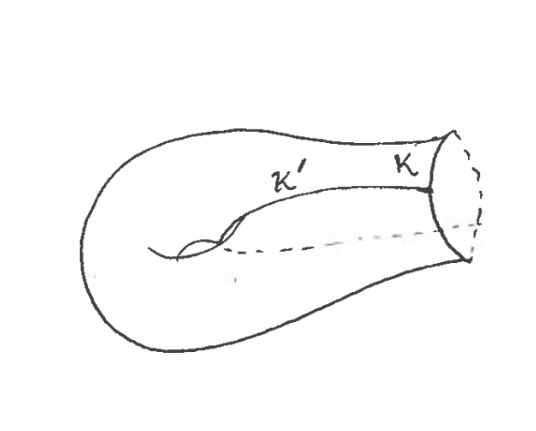
\includegraphics[height=5cm]{images/s101-draft.png}
      \caption{({\color{red} Draft})The curves $\kappa$ and $\kappa^{\prime}$ on $\os_{1,0,1}$.}
      \label{fig:base-case-2}
    \end{figure}

    From the previous case, we already have $\hNP(\core(\teich(\os_{1,1,0}))) = \hLP(\teich(\os_{1,1,0}))$, and since their mapping class groups are isomorphic, we also have $\hLP(\teich(\os_{1,1,0})) = \hLP(\teich(\os_{1,0,1}))$.
    We now need to prove that $\hNP(\core(\teich(\os_{1,1,0}))) = \hNP(\core(\teich(\os_{1,0,1})))$ to prove the result for this case.
    We have that the net for $\core(\teich(\os_{1,0,1}))$ lies in a bounded neighbourhood of the net for $\core(\teich(\os_{1,1,0}))$: this implies that the cardinalities of the net points in a ball of radius $r$ differ by at most a multiplicative constant.
    \begin{align*}
      \#\left( B_R(p) \cap \net_{\core(\teich(\os_{1,0,1}))} \right) \leq c \cdot \#\left( B_R(p) \cap \net_{\core(\teich(\os_{1,1,0}))} \right)
    \end{align*}
    Since the two cardinalities differ by at most a multiplicative constant, they have the same exponential growth rate.
    % The equality of $\hLP(\teich(\os_{1,0,1}))$ and $\hNP(\core(\teich(\os_{1,0,1})))$ follows from the equality for $\os_{1,1,0}$ {\color{red} (Maybe add a lemma here that states that the entropy stays equal if you take a bounded neighbourhood)}.
  \item $\os_{0,2,1}$: The mapping class group of this surface is finite: in fact, it is isomorphic to $\mathbb{Z}/2\mathbb{Z} \times \mathbb{Z}/2\mathbb{Z}$ (see \textcite{gendulphe2017whats}).
    This means $\hLP(\teich(\os_{0,2,1})) = 0$.
    This surface has exactly two simple geodesics $\kappa$ and $\kappa^{\prime}$, which intersect each other exactly once, such that deleting either one of them results in a pair of pants.
    Picking a pants decomposition along either $\kappa$ or $\kappa^{\prime}$, we see that $\teich(\os_{0,2,1})$ is homeomorphic to $\mathbb{R}_{>0}$, where the homeomorphism is given by the length coordinate.

    If we now consider $\core(\teich(\os_{0,2,1}))$, the lengths of $\kappa$ and $\kappa^{\prime}$ are bounded below by the threshold.
    But they are also bounded above, by an argument similar to the previous case, namely is either $\kappa$ or $\kappa^{\prime}$ are very long, the other one sided curve must be very short.
    This proves that $\core(\teich(\os_{0,2,1}))$ is compact, and as a result $\hNP(\core(\os_{0,2,1})) = 0$.
    This proves the lemma for $\os_{0,2,1}$.
  \item $\os_{0,1,2}$: This surface has a unique two-sided element, which we denote by $\gamma_{\infty}$.
    The one sided curves on this surface are indexed by $\mathbb{Z}$, where $\gamma_n = D_n \gamma_0$, and $D_n$ is the Dehn twist about $\gamma_\infty$.
    The mapping class group of this surface is also virtually generated by $D_n$.
    If we consider the pants decomposition along $\gamma_{\infty}$, we get a Fenchel-Nielsen map from $\teich(\os_{0,1,2})$ to the upper half plane $\mathbb{H}^2$, where the $y$-coordinate is $\frac{1}{\ell(\gamma_{\infty})}$, and the $x$-coordinate is the twist around $\gamma_{\infty}$.
    Furthermore, this map is also an isometry, and with respect to these coordinates, $D_n$ is the action of $
    \begin{pmatrix}
      1 & 1 \\
      0 & 1
    \end{pmatrix}
    $ on $\mathbb{H}^2$.

    If we now consider $\core(\teich(\os_{0,1,2}))$, that consists of the points in $\mathbb{H}^2$ whose $y$-coordinate is greater than some threshold value, i.e. a horoball in $\mathbb{H}^2$.
    We know from elementary hyperbolic geometry that the number of net points in a horoball grows with the same exponential growth rate as the number of net points in the boundary of the horoball, i.e. the horocycle.
    The former exponential growth rate is precisely $\hNP(\core(\teich(\os_{0,1,2})))$, and the latter term is $\hLP(\teich(\os_{0,1,2}))$.
  \end{itemize}
  This concludes the proof of the lemma for the $4$ surfaces with $\chi(S) = -1$.
\end{proof}

\subsection{Good points and bad points}
\label{sec:good-points-bad}

The proof of Theorem \ref{thm:entropy-equality} will split up into counting two kinds of net points, which we will call \emph{good points} and $\emph{bad points}$.

\begin{definition}[Good points]
  A point in $B_R(p) \cap \net$ is good if it is at most distance $\vepb R$ away from a lattice point $\gamma p$. The set of good points is denoted by $\net_g(p, R, \vepb)$.
\end{definition}

\begin{definition}[Bad points]
  A point in $B_R(p) \cap \net$ is bad if it is more than distance $\vepb R$ away from the nearest lattice point. The set of bad points is denoted by $\net_b(p, R, \vepb)$.
\end{definition}

Observe that the classification of a point as good or bad depends on the choice of $R$, $p$, and an additional parameter $\vepb > 0$.

We also further subdivide $\net_g(p, R, \vepb)$ based on what the closest lattice point is.

\begin{definition}[Good point in the domain of $\gamma$]
  For $\gamma \in \mcg(S)$, the set $\net_g(\gamma, p, R, \vepb)$ denotes the subset of $\net_g(p, R, \vepb)$ whose closest lattice point is $\gamma p$.
\end{definition}

We will now prove a lemma that provides an upper bound on the number of good points when restricted to a fundamental domain.

\begin{lemma}
  \label{lem:fd-polynomial-growth}
  There exists a polynomial function $q$, whose degree only depends on the topological type of $S$, such that for any $\gamma \in \mcg(S)$, the following inequality holds for the cardinality of points in $\net_g(\gamma, p, R, \vepb)$.
  \begin{align*}
    \#\left( \net_g(\gamma, p, R, \vepb) \cap B_R(\gamma p) \right) \leq q(R)
  \end{align*}
\end{lemma}

\begin{rem}
  \textcite[Lemma 3.2]{eskinmirzakhani} prove this lemma for Teichmüller spaces of orientable surfaces, by comparing the extremal lengths of various curves on the underlying surfaces.
  We adapt the same proof for non-orientable surfaces, replacing extremal length for hyperbolic lengths instead.
\end{rem}

Before we prove Lemma \ref{lem:fd-polynomial-growth}, we will need the following lemma on packing an $\vepn$-separated set into a ball of fixed radius in Teichmüller space (where $\vepn$ is the parameter associated to our net $\net$).

\begin{lemma}[Packing bound]
  \label{lem:packing-argument}
  For an constants $C > 0$ and $\vepn > 0$, there exists a constant $D(C, \vepn, S)$ depending on the constants $C$, $\vepn$, and the topological type of the surface $S$ such that any ball $B_C(p)$ (independent from the choice of $p$) in $\teich(S)$ cannot contain more than $D$ points that are pairwise distance at least $\vepn$ apart.
\end{lemma}

\begin{proof}
  First of all, note that the above lemma holds for $S = \os_{1,1,0}$, since $\teich(\os_{1,1,0})$ is $\mathbb{H}^2$, which is homogeneous.

  Next, note that the lemma also holds for compact metric spaces, because we can express $D$ as a continuous function of the point $p$, which will achieve a maximum on a compact metric space.

  Finally, note that if the lemma holds for metric spaces $X$ and $Y$, it also holds for $X \times Y$, where the metric on $X \times Y$ is the $\sup$ product with an additive error.

  Suppose now that we have the lemma for the Teichmüller spaces of all surfaces with Euler characteristic at least $-n$.
  To show the lemma for a Teichmüller space of a surface $S$ with Euler characteristic $-n-1$, we break up the Teichmüller space into the thick part, where the mapping class group acts co-compactly, so the first reduction applies, and the thin part, where we have by Minsky's product region theorem \cite[Theorem 6.1]{1077244446} (or Theorem \ref{thm:prno}), the metric is the $\sup$ product, so the second reduction applies.
\end{proof}

\begin{proof}[Proof of Lemma \ref{lem:fd-polynomial-growth}]
  We begin by making three simplifying reductions.
  First, it will suffice to prove the following stronger claim instead.
  \begin{align}
    \label{eq:reduction-one}
    \#\left( \net(\gamma) \cap B_R(\gamma p) \right) \leq q(R)
  \end{align}
  Here, $\net(\gamma)$ denotes the set of net points whose closest lattice point is $\gamma p$: $\net(\gamma)$ is therefore a superset of $\net_g(\gamma, p, R, \vepb)$.

  Next, note that it suffices to prove \eqref{eq:reduction-one} for $\gamma = 1$, since our choice of basepoint $p$ was arbitrary.

  And finally, it will suffice to prove the following claim.
  \begin{claim*}
  There exists a set $\cZ \subset \teich(S)$ such that $\# \cZ \leq R^{f(S)}$, and for $y \in B_R(p)$, there exists a $z \in \cZ$ and $\kappa \in \mcg(S)$ such that $d(y, \kappa z) \leq C$, for some value $f(S)$ that only depends on the topological type of $S$, and some fixed constant $C$.
  \end{claim*}
  To see why this suffices, suppose we have such a $\cZ$.
  Without loss of generality, we can assume that for all points $z \in \cZ$, the closest lattice point is $p$: otherwise we could replace such a point $z$ by $\kappa z$ for an appropriate choice of $\kappa$.
We then have that for any $n \in \net(1) \cap B_p(R)$, there exists some $z \in \cZ$, such that $d(z, n) \leq C$.
Since $\# \cZ \leq R^{f(\chi(S))}$, we have that $\#\left( \net(1) \cap B_p(R) \right) \leq C^{\prime} R^{f(\chi(S))}$, for some other constant $C^{\prime}$, by Lemma \ref{lem:packing-argument}.
% \todo[inline]{Need a lemma that states we can only pack in a uniformly bounded number of net points in a ball of fixed radius.
% The proof can go via the uniform Lagrangian estimate for the volume of a ball, and use packing arguments.}

\emph{Proof of claim:}
  Let $\left\{ M_1, \ldots, M_J \right\}$ be all the topologically distinct markings on $p$ that are short.
  We know that there are only finitely many of them, and the cardinality $J$ only depends on the topological type of the surface $S$.
  We also know that for each of these short markings, the lengths of the pants curves in the marking are bounded above by some constant $T$.
  Each of these markings has $N = -3 \chi(S) - b$ pants curves on them, where $b$ is the number of boundary components of $S$.

  We construct the points $z \in \cZ$ by just varying the lengths of these pants curves: the set of lengths we will allow are the following.
  \begin{align*}
    \text{Acceptable lengths} = \left\{ T, T \exp(-1), T\exp(-2), \ldots, T \exp(-\lceil R \rceil) \right\}
  \end{align*}
  We define the point $z_{j, i_1, i_2, \ldots , i_N}$ to be the point in $\teich(S)$ obtained by considering the marking $M_j$ at $p$, and setting the length of the $k$\textsuperscript{th} pants curve to be $i_k$, where the $i_k$ is one of the acceptable lengths.
  It's clear that the cardinality of $\cZ$ is at most $J \cdot R^N$, which is a polynomial only depending on the topological type of the surface $S$.

  Suppose now that $y$ is some other point in $B_R(p)$.
  We pick a $\kappa \in \mcg(S)$ such that the shortest marking on $\kappa y$ is one of the markings $M_j$ for $1 \leq j \leq J$.
  We now need to show that one of the $z \in \cZ$ is close to $\kappa y$.
  Pick the $z$ such that the corresponding lengths of the pants curves are closest to the lengths of the pants curves on $\kappa y$.
  We can now invoke the combinatorial distance formula for Teichmüller metric (proved by \textcite{rafi2007combinatorial} for the orientable setting, and Theorem \ref{thm:distance-formula} for the non-orientable case).
  \begin{align*}
    d(z, \kappa y) \emul \sum_Y \left[ d_Y(z, \kappa y) \right]_k + \sum_{\alpha \not \in \Gamma} \log \left[ d_{\alpha} (z, \kappa) \right]_k + \max_{\alpha \in \Gamma} d_{\mathbb{H}_{\alpha}} (z, \kappa y)
  \end{align*}
  In the above formula, the first term is the distance between the short markings when projected to non-annular subsurfaces, the second term is the distance between the short markings when projected to annular subsurfaces whose core curves are not the pants curves in the marking, and the third term corresponds to the length and twist parameters of the short curves.

  Since both $z$ and $\kappa y$ have the same short markings, the first two terms in the above sum become $0$.
  Also, since we picked $z$ to be the element of $\cZ$ such that the lengths were closest to those on $\kappa y$, the third term is bounded by some constant, which proves the result.
\end{proof}


\subsection{Using complexity length to count bad points}
\label{sec:using-compl-length}

In this section we introduce an alternative to the Teichmüller metric, called the \emph{complexity length} (see Definition \ref{defn:complexity-length}).
This metric was introduced by \textcite{dowdall2023lattice}, in order to get better estimates on net points contained in the thin part of Teichmüller space (for orientable surfaces).
We adapt the construction of complexity to the Teichmüller space of non-orientable surfaces in Section \ref{sec:line-gap-compl}.
In this section, we state the main results about complexity length we need in order to prove Theorem \ref{thm:entropy-equality}.

For this section, we will state the results with a rescaled version of complexity length, in order to compare it with Teichmüller length.

\begin{definition}[Rescaled complexity length]
  Let $S$ be a surface of finite type.
  The rescaled complexity length $\dcomp$ on $\core(\teich(S))$ is given by the following formula.
  \begin{align*}
    \dcomp(x, y) = \frac{\mathfrak{L}(x,y)}{\hNP(\core(\teich(S)))}
  \end{align*}
  Here, $\mathfrak{L}(x,y)$ is the complexity length between points $x$ and $y$.
\end{definition}

The first result we will need is a count of the net points with respect to the rescaled complexity length.

\begin{theorem}[Theorem 12.1 of \cite{dowdall2023lattice}, Theorem \ref{thm:counting-with-complexity}]
  \label{thm:counting-with-complexity-rescaled}
  There exists a polynomial function $p(R)$ that depends on the net $\net$, and a parameter $\veperr > 0$, such that the following inequality holds for any $\veperr > 0$.
  \begin{align*}
    \#\left( y \in \net \mid \dcomp(p, x) \leq R \right) \leq p(R) \exp((\hNP(\core(\teich(S))) + \veperr) \cdot R)
  \end{align*}
\end{theorem}
% \todo[inline]{Add the $\varepsilon_1$ parameter.}

The next result, which is the main theorem of Section \ref{sec:line-gap-compl}, is that if $y$ is a bad point that is Teichmüller distance $R$ away from $p$, then its rescaled complexity distance to $p$ is smaller than $R$ by a definite amount.
We state this theorem with an additional hypothesis on the net point entropy of subsurfaces.
We will establish that this hypothesis holds inductively in Section \ref{sec:proof-theorem}.

\begin{theorem}[Linear gap in complexity length, Theorem \ref{thm:linear-gap}]
  \label{thm:linear-gap-rescaled}
  Suppose that for all proper subsurfaces $V$ of $\os$, the following inequality holds.
  \begin{align*}
    \hNP(\core(\teich(V))) < \hNP(\coret{\os})
  \end{align*}
  Then for any $\vepb >0$, there exists $c > 0$, such that for any bad point $y$, i.e. a point in $\net_b(p, R, \vepb)$, the following upper bound on the complexity distance between $p$ and $y$ holds.
  \begin{align*}
    \dcomp(p, y) \leq R(1 - c)
  \end{align*}
\end{theorem}
\begin{rem}
  We give a brief outline of why the above result should hold.
  Complexity length can be thought of as a weighted version of Teichmüller length, where a specific segment is assigned a weight based on whether it's traveling in the thick part of Teichmüller space, or the thin part.
  In the latter case, it is assigned a smaller weight that is proportional to the net point entropy of the product region it is traveling in.
  The Teichmüller geodesics associated to bad points spend a significant fraction traveling in the thin part, by the very definition of bad points.
  It stands to reason then that the complexity length assigned to them is smaller by a definite amount, due to the time they spend in the thin part.
\end{rem}
% \todo[inline]{Have a remark here on why this ought to be true.}

Combining Theorems \ref{thm:counting-with-complexity-rescaled} and \ref{thm:linear-gap-rescaled}, it follows that as $R$ goes to $\infty$, the proportion of bad points goes to $0$, which is what we need for Theorem \ref{thm:entropy-equality}.

\subsection{Entropy gap}
\label{sec:entr-gap-cons}

In the previous section, we saw that the key hypothesis we need for the complexity length estimate was that for any proper subsurface $V$ of $\os$, the following strict inequality held.
\begin{align}
  \label{eq:net-point-entropy-gap}
  \hNP(\core(\teich(V))) < \hNP(\coret(\os))
\end{align}

In this section, we will prove that \eqref{eq:net-point-entropy-gap} holds by proving a similar inequality for the lattice point entropy, and using the fact that Theorem \ref{thm:entropy-equality} holds for all proper subsurfaces $V$, by the inductive hypothesis.

\begin{lemma}[Lattice point entropy gap]
  \label{lem:entropy-inequality}
  Let $\os$ be a surface, and $\chi(\os) \leq -2$. If $V$ is a proper subsurface and Theorem \ref{thm:entropy-equality} holds for $V$, then we have the following strict inequality between their lattice point entropy.
  \begin{align*}
    \hLP(\teich(V)) < \hLP(\teich(\os))
  \end{align*}
\end{lemma}

\begin{rem}
  We do actually need the hypothesis $\chi(\os) \leq -2$ in the statement of the lemma for two reasons.
  The first reason is that the lemma is actually false for $\os_{1,0,1}$.
  Recall that this surface has the torus with one boundary component as a subsurface, but their mapping class groups are isomorphic, and have the same lattice point growth entropy.
  Another reason why we need the hypothesis is that the proof of the lemma proceeds via a construction of pseudo-Anosov elements on $\os$, and $\os_{1,0,1}$ does not admit any pseudo-Anosov mapping classes.
\end{rem}

\begin{proof}[Proof of Lemma \ref{lem:entropy-inequality}]
  Observe that $\mcg(V)$ is a subgroup of $\mcg(\os)$.
  We will first construct an intermediate subgroup $H = \mathbb{Z} * \mcg(V)$, which is the free product of a psuedo-Ansov element in $\mcg(\os)$ with $\mcg(V)$, and show that $\hLP(H) > \hLP(\mcg(V))$.
  This is enough to prove the result, since $H$ is a subgroup of $\mcg(\os)$, we have that $\hLP(\mcg(\os)) \geq \hLP(H)$.

  We now need to show that $\mcg(\os)$ contains a pseudo-Anosov element.
  We can invoke Penner's construction of pseudo-Anosov mapping classes (\cite[Theorem 4.1]{penner1988construction}), as long as we can construct a filling collection of \emph{two-sided} curves in $\os$.
  This may not be always possible for $\os$ where $\chi(\os) = -1$, but for $\os$ with $\chi(\os) \leq -2$, this is always possible (see \cite{Liechti2018MinimalPS} and \cite{khan2023pseudo} for explicit constructions).
  Let $\kappa$ denote the pseudo-Anosov mapping class we construct.

  We have that the expanding and contracting foliations of $\kappa$ are disjoint fromt the limit set of $\mcg(V)$ in the Thurston boundary.
  This is because the limit set of $\mcg(V)$ can only consist of foliations supported on the subsurface $V$, whereas the expanding and contracting foliations of $\kappa$ fill the entire surface.
  We can now invoke the ping-pong lemma to conclude that the group generated by a large enough power of $\kappa$ and $\mcg(V)$ is the free product of $\mathbb{Z}$ and $\mcg(V)$: we let $H$ denote this group.

  We now need to show that the lattice point entropy for $H$ is strictly larger than the $\mcg(V)$.
  To see this, we recall an equivalent definition of the lattice point entropy.
  The lattice point entropy is the parameter $h$ such that the following Poincaré series transitions from being convergent to divergent for any $x \in \teich(\os)$.
  \begin{align}
    \label{eq:dirichlet}
    \sum_{\gamma \in H} \exp\left( -h \cdot d(x, \gamma x) \right)
  \end{align}
  Since $H = \mathbb{Z} * \mcg(V)$, we can represent $\gamma \in H$ as $a_1 \cdot b_1 \cdot a_2 \cdots a_k \cdot b_k$, where $a_i$ belong in $\mathbb{Z}$ and $b_i$ belong in $\mcg(V)$.
  We use this along with the triangle inequality to get an upper bound for $d(x, \gamma x)$.
  \begin{align}
    \label{eq:triangle-inequality-1}
    d(x, \gamma x) \leq \sum_{i=1}^k d(x, a_i x) + d(x, b_i x)
  \end{align}
  We plug inequality \eqref{eq:triangle-inequality-1} into \eqref{eq:dirichlet} to get a lower bound.
  \begin{align}
    \label{eq:dirichlet-lower-bound}
    \sum_{\gamma \in H} \exp\left( -h \cdot d(x, \gamma x) \right) &= \sum_{k=1}^\infty \left(  \sum_{a_1}\cdots \sum_{a_k} \sum_{b_1}\cdots \sum_{b_k}  \exp(-h \cdot d(x, a_1 \cdot b_1 \cdots a_k \cdot b_k x)) \right) \\
    &\geq \sum_{k=1}^{\infty} \left( \sum_{a \in \mathbb{Z}} \exp(-h \cdot d(x, ax)) \right)^k \left( \sum_{b \in \mcg(V)} \exp(-h \cdot d(x, bx)) \right)^k
    \label{eq:dirichlet-lower-bound-2}
  \end{align}

  We have that Theorem \ref{thm:entropy-equality} holds for $V$, which means that $\core(\teich(V))$ is SCC.
  Corollary 5.4 of \cite{10.1093/imrn/rny001} states that group actions that are SCC have Poincaré series that diverge at the critical exponent.
  This means there's small enough $\varepsilon > 0$ such that for $h = \hLP(\teich(V)) + \varepsilon$, the series converges to a value greater than $1$.
  But that means the Poincaré series for $H$ diverges at $\hLP(\teich(V)) + \varepsilon$, since we have a lower bound by a geometric series whose ratio is greater than $1$.
  This proves that the critical exponent for $H$ is strictly greater than the critical exponent for $\mcg(V)$.
\end{proof}

We can now prove the entropy gap result for $\hNP$.

\begin{lemma}[Net point entropy gap]
  \label{lem:net-point-entropy-inequality}
  Let $\os$ be a surface, and $\chi(\os) \leq -2$. If $V$ is a proper subsurface and Theorem \ref{thm:entropy-equality} holds for $V$, then we have the following strict inequality between their net point entropy.
  \begin{align*}
    \hNP(\core(\teich(V))) < \hNP(\core(\teich(\os)))
  \end{align*}
\end{lemma}

\begin{proof}
  We have the following inequality, which follows trivially from the definition of $\hLP$ and $\hNP$.
  \begin{align}
    \label{eq:ineq1}
    \hLP(\teich(\os)) \leq \hNP(\core(\teich(\os)))
  \end{align}
  From Lemma \ref{lem:entropy-inequality}, we get the following inequality.
  \begin{align}
    \label{eq:ineq2}
    \hLP(\teich(V)) < \hLP(\teich(\os))
  \end{align}
  Finally, since we have Theorem \ref{thm:entropy-equality} for $V$, we have the following equality.
  \begin{align}
    \label{eq:eq3}
    \hLP(\teich(V)) = \hNP(\core(\teich(V)))
  \end{align}
  Chaining together \eqref{eq:ineq1}, \eqref{eq:ineq2}, and \eqref{eq:eq3} gives us the result.
\end{proof}

\subsection{Proof of Theorem \ref{thm:entropy-equality}}
\label{sec:proof-theorem}

We now have all the lemmas we need in order to prove Theorem \ref{thm:entropy-equality}.

\begin{proof}[Proof of Theorem \ref{thm:entropy-equality}]
  We will prove this lemma by inducting on the complexity of the surface $\os$.
  Lemma \ref{lem:entropy-equality-base-case} proves the result for surfaces with Euler characteristic equal to $-1$, which serves as the base case of the theorem.

  We now assume that Theorem \ref{thm:entropy-equality} already holds for all proper subsurfaces $V$ of $\os$: it will suffice to show that the result holds for $\os$.

  We will establish that for any $\vepb > 0$, there exists a polynomial $q(R)$, and $R$ large enough, such that the following bound holds.
  \begin{align*}
    \#\left( B_R(p) \cap \net \right) \leq q(R) \cdot \exp(\hLP(\teich(\os)) \cdot R \cdot (1 + 2 \vepb))
  \end{align*}

  We first count the good points in $B_R(p)$, by partitioning them according to the nearest lattice point.
  \begin{align}
    \label{eq:good-point-partition}
    \net_g(p, R, \vepb) = \bigsqcup_{\gamma \in \mcg(\os)} \net_g(\gamma, p, R, \vepb)
  \end{align}
  Observe that if $y \in \net_g(\gamma, p, R, \vepb)$, then $d(p, \gamma p) \leq R(1 + \vepb)$, since $d(p, y) \leq R$ and $d(y, \gamma p) \leq \vepb R$.
  This observation leads to the following upper bound on $\#\left( \net_g(p, R, \vepb) \right)$.
  \begin{align}
    \#\left( \net_g(p, R, \vepb) \right) \leq \sum_{\substack{\gamma \in \mcg(\os) \\ d(p, \gamma p) \leq R(1 + \vepb)}} \#\left( B_{\vepb R}(\gamma p) \cap \net_g(\gamma, p, R, \vepb)  \right) \label{eq:good-estimate-1}
  \end{align}
  By Lemma \ref{lem:fd-polynomial-growth}, there exists a polynomial $q(R)$ such that each term in the above sum is at most $q(R)$.
  \begin{align}
    \#\left( \net_g(p, R, \vepb) \right) &\leq \sum_{\substack{\gamma \in \mcg(\os) \\ d(p, \gamma p) \leq R(1 + \vepb)}} q(R) \\
     &\leq q(R) \cdot \exp(\hLP(\teich(\os)) \cdot R \cdot (1 + 2 \vepb))
    \label{eq:good-estimate-2}
  \end{align}
  Here, we estimated the cardinality of $\gamma$ such that $d(p, \gamma p) \leq R(1+\vepb)$ as at most $\exp(\hLP(\teich(\os)) \cdot R \cdot (1 + 2 \vepb))$, for large enough $R$.
  We have the desired upper bound on the cardinality for the good points.
  Now we show that the number of bad points is much smaller than the total number of points in the ball, which will then prove the result.

  From the inductive hypothesis, we have that Theorem \ref{thm:entropy-equality} holds for all proper subsurfaces $V$.
  By Lemma \ref{lem:net-point-entropy-inequality}, we have that $\hNP(\core(\teich(V))) < \hNP(\core(\teich(\os)))$: this is precisely the hypothesis we need to apply Theorem \ref{thm:linear-gap-rescaled}.
  Applying the theorem, we see that if $y$ is a bad point, $\dcomp(p, y) \leq R(1 - c)$.
  We then apply Theorem \ref{thm:counting-with-complexity-rescaled} to get an upper bound on the number of bad points.
  \begin{align*}
    \#\left( \net_b(p, R, \vepb) \right) \leq kR^k \cdot \exp((\hNP(\core(\teich(\os))) + \veperr) \cdot R \cdot (1 - c))
  \end{align*}
  We pick $\veperr$ small enough such that the above term satisfies the following inequality for large enough $R$.
  \begin{align*}
    \exp((\hNP(\core(\teich(\os))) + \veperr) \cdot R \cdot (1 - c)) < \exp\left(\hNP(\core(\teich(\os))) \cdot R \cdot \left(1 - \frac{2c}{3}\right)\right)
  \end{align*}
  On the other hand, we have that for large enough $R$, the total number of net points is at least $\exp\left(\hNP(\core(\teich(\os))) \cdot R \cdot \left(1 - \frac{c}{2}\right)\right)$.
  Combining these two facts, we see that the proportion of bad points goes to $0$ as $R$ goes to $\infty$, which proves the result.
\end{proof}
% \todo[inline]{Change wherever you've used $N$ to $\net$.}

% Before we state the various lemmas we will need for the proof of the inductive step, we sketch the outline of the proof, to illustrate the key idea of the proof, as well as enumerate the difficulties in proving the result.

% \begin{proof}[Proof sketch of Theorem \ref{thm:entropy-equality}]
%   It will suffice to prove the following upper bound for any $\varepsilon > 0$ and for large enough $R$, and some polynomial function $q$.
%   \begin{align*}
%     \#\left( B_R(p) \cap N \right) \leq q(R) \cdot \exp(\hLP R (1 + 2\varepsilon))
%   \end{align*}
%   We do this by partitioning the points in $B_R(p) \cap N$ into two sets.
%   \begin{description}
%   \item[Good points] The points in $B_R(p) \cap N$ which are at most distance $\varepsilon R$ away from the closest lattice point.
%     We denote this by $N_g(p, R)$, since the definition of goodness also depends on $p$ and $R$.
%   \item[Bad points] The points in $B_R(p) \cap N$ which are more than distance $\varepsilon R$ away from the closest lattice point.
%     We denote these points by $N_b(p, R)$.
%   \end{description}
%   \todo[inline]{Factor out this definition outside the proof sketch.}

%   The first step of the proof is to get an upper bound on the number of good points.
%   To each point in $B_R(p) \cap N$, we associate the nearest lattice point $\gamma p$.
%   Let $N(\gamma)$ denote the subset of net points whose closest lattice point is $\gamma p$.
%   Observe that if $x \in N(\gamma)$ is a good point, i.e. is contained in $N_g(p, r)$, then $d(p, \gamma p)$ is at most $R + \varepsilon R$, by the triangle inequality.
%   This observation leads us to the following estimate for $\#\left( N_g(p, r) \right) $.
%   \begin{align}
%     \#\left( N_g(p, r) \right) \leq \sum_{\substack{\gamma \in \mcg(\os) \\ d(p, \gamma p) \leq R(1 + \varepsilon)}} \#\left( B_{\varepsilon R}(\gamma p) \cap N(\gamma)  \right) \label{eq:good-estimate-1}
%   \end{align}

%   The next step in the proof is to show that $\#\left(  B_{\varepsilon R}(\gamma p) \cap N(\gamma)  \right)$ has polynomial growth as $R$ increases: this is the content of Lemma \ref{lem:fd-polynomial-growth}.
%   Using this estimate, we can rewrite \eqref{eq:good-estimate-1} in terms of the lattice point counting function for large enough values of $R$.
%   \begin{align}
%     \label{eq:good-estimate-2}
%     \#\left( N_g(p, r) \right) &\leq q(R) \cdot \#\left( \gamma \in \mcg(\os) \mid d(p , \gamma p) \leq R(1 + \varepsilon) \right) \\
%     &\leq q(R) \cdot \exp\left( \hLP R(1 + 2\varepsilon) \right)
%     \label{eq:good-estimate-3}
%   \end{align}
%   \todo[inline]{Need to adapt the proof of  \cite[Lemma 3.2]{eskinmirzakhani}.}

%   This proves the estimate we want for the set of good points.
%   To deal with the bad points, we will show that as $R$ gets larger, the fraction of bad points in $B_R(p) \cap N$ goes to $0$.
%   This will show that the estimate we got for good points in \eqref{eq:good-estimate-3} holds for all points in $B_R(p) \cap N$, for large enough $R$.

%   To show that the fraction of bad points goes to $0$, we count with respect to a new metric $d_C$, instead of the Teichmüller metric.
%   This new metric is called complexity length (\textcite{dowdall2023lattice}), and one has a similar lattice point counting result with respect to this new metric for large enough $R$.
%   \begin{align}
%     \#\left( n \in N \mid d_C(p, n) \leq R \right) \leq \exp((\hNP + \delta) R)
%     \label{eq:complexity-length-count}
%   \end{align}
%   Here, $\delta$ is some arbitrary positive constant, and picking a smaller $\delta$ means one has to pick a larger value of $R$ to make the above inequality hold.

%   The main reason we work with complexity length instead of the Teichmüller metric is that we can get a better estimate for complexity length for bad points: this is the content of Theorem \ref{thm:complexity-length-gap}.
%   For a point $n \in N_b(p, R)$, we have the following estimate for $d_C(p, n)$, for some constant $c > 0$.
%   \begin{align*}
%     d_C(p, n) \leq R(1 - c \varepsilon)
%   \end{align*}
%   Combining the above inequality with \eqref{eq:complexity-length-count} for a small enough $\delta$, we get that the fraction of bad points goes to $0$ as $R$ goes to $\infty$.
% \end{proof}

% Before we prove the induction step of the argument, we state a few lemmas that will go into the proof.

\section{Linear gap in complexity length}
\label{sec:line-gap-compl}

\subsection{An example of counting in product regions}
\label{sec:an-example-counting}

Before we define complexity length, we will look at an example that illustrates why we need complexity length.
Theorem 1.3 of \textcite{10.1215/00127094-1548443} proves an estimate on the volume of balls in Teichmüller space.
From this volume estimate, we can obtain an estimate on the cardinality of net points of an $(\vepn, 2 \vepn)$-net $\net$.
\begin{theorem}[Theorem 1.3 of \cite{10.1215/00127094-1548443}]
  \label{thm:abem}
  For a point $p$ in $\teich(S)$ (where $S$ is a genus $g$ surface with $b$ boundary components), the number of net points in a ball of radius $R$ centered at the origin satisfies the following asymptotic as $R$ goes to $\infty$.
  \begin{align*}
    \#\left( \net \cap B_R(p) \right) \emul \exp((6g-6 + 2b)R)
  \end{align*}
  Here, the multiplicative and additive constants showing up in $\emul$ only depend on $p$ and $\vepn$.
\end{theorem}

Suppose now that we want to use the above theorem to count net points in a product region.
More concretely, let $p$ be a point in $\teich(S)$ such that a non-separating curve $\gamma$ is very short: $\ell_{\gamma}(p) \leq \delta \cdot \exp(-R_0)$, for some $\delta > 0$, and some large $R_0$, and we want to estimate the cardinality of $\net \cap B_R(p)$ for $R < R_0$.
Note that since $R < R_0$, the ball $B_R(p)$ is still contained in the product region of Teichmüller space where $\ell_\gamma \leq \delta$.

Since the entire ball $B_R(p)$ is in a product region, we have by Minsky's product region theorem (see Theorem \ref{thm:prno} for a precise statement) that the ball decomposes (up to an additive error) as the
product of a ball in $\teich(S \setminus \gamma)$ and ball in $\mathbb{H}$ (which corresponds to the length and twist around $\gamma$).
This gives us an alternative estimate for $\#\left( \net \cap B_R(p)\right)$.
\begin{align}
  \label{eq:prod-decomp}
  \#\left( \net \cap B_R(p) \right) &\leq C \cdot \left( \net_1 \cap B_R(p, S \setminus \gamma) \right) \cdot \left( \net_2 \cap B_R(p, \mathbb{H})\right)
\end{align}
Here $\net_1$ and $\net_2$ are $(\vepn, 2\vepn)$ nets for $\teich(S \setminus \gamma)$ and $\mathbb{H}$, and $B_R(p, S \setminus \gamma)$ and $B_R(p, \mathbb{H})$ are projections on the ball $B_R(p)$ to the two components.
Applying Theorem \ref{thm:abem} to the right hand side of \eqref{eq:prod-decomp}, we get a better estimate than we would have gotten with a direct application of Theorem \ref{thm:abem}.
\begin{align*}
  \#\left( \net \cap B_R(p) \right) &\leq C \cdot \left( \net_1 \cap B_R(p, S \setminus \gamma) \right) \cdot \left( \net_2 \cap B_R(p, \mathbb{H})\right) \\
                                           &\emul \exp((6(g-1)-6 + 2(b+2))R) \cdot \exp(R) \\
  &= \exp((6g-6+2b-1)R)
\end{align*}

This example illustrates that in order to count net points accurately, it's not sufficient to just estimate the distance the between the base point $p$ and the net point $n$: if the geodesic segment $[p, n]$ travels in a product region, the count will be lower than what Theorem \ref{thm:abem} predicts.
In fact, the count will also depend on the type of the product region.
In the above example, the product region had just one curve $\gamma$ becoming short, but in general, a product region can have multiple curves getting short, in which case, the net point count will be even smaller.

We now consider a geodesic $[x,y]$ (where $x$ and $y$ are net points) that travels through several product regions $p_i$, and possibly the thick part, which we will also consider a product region, albeit a trivial one.
Let $h_i$ be the exponent associated to the product region $p_i$: this is the exponent that will appear when we invoke Theorem \ref{thm:abem} to count net points in the product region $p_i$.
The order in which $[x, y]$ travels through the product region is specified in \autoref{fig:schematic}.
\begin{figure}[h]
  \centering
  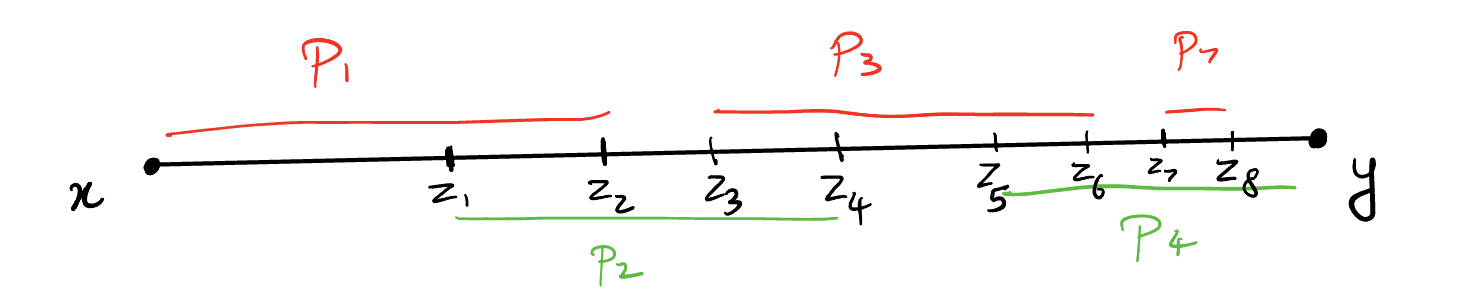
\includegraphics[scale=0.5]{images/schematic.png}
  \caption{A schematic of the geodesic $[x,y]$ traveling through several product regions.}
  \label{fig:schematic}
\end{figure}

Let $z_i$ denote the points on the geodesic segment that correspond to the times when the geodesic enters or exits a product region: in \autoref{fig:schematic}, we have labeled $z_i$ for $1 \leq i \leq 8$.
Let $\mathcal{J}_i$ denote the interval $[x, z_1]$ for $i=0$, the interval $[z_i, z_{i+1}]$ for $1 \leq i \leq 7$, and $[z_8, y]$ for $i=8$.
Let $\ell_i$ be the length of $\mathcal{J}_i$, and $e_i$ be the sum of the $h_i$ for each of the product regions that the interval $\mathcal{J}_i$ is in.
Also, for each $z_i$, let $z_i^{\prime}$ denote the nearest net point.

Keeping $x$ fixed, we can try to count the number of net points $y$ that satisfy the configuration we have described.
We have about $O(\exp(e_0 \ell_0))$ possibilities for $z_1^{\prime}$, and then keeping a $z_1^{\prime}$ fixed, $O(\exp(e_i \ell_1))$ possibilities for $z_2^{\prime}$ and so on.
Multiplying all these estimates, we have the following upper bound for cardinality of $y$.
\begin{align*}
  \#\left( y \right) \leq \exp\left( \sum_{i=0}^8 e_i \ell_i \right)
\end{align*}

The quantity $\sum e_i \ell_i$ serves as a re-weighted version of length of the geodesic in manner that works well with the counting function.
This is a primitive version of the \emph{complexity length} of $[x,y]$, and motivates the actual definition.

Before we define complexity length, we note two ways in which the above estimate overestimates the actual number of net points: that happens when a point in the geodesic is simultaneously in two or more product regions, which can happen in two ways.
\begin{enumerate}[(i)]
\item The product regions are disjoint: In this case, we are accounting the length of the geodesic segment multiple times: once for each product region we are in. However, this overcounting is still better than directly invoking Theorem \ref{thm:abem}, since the sums of the exponents $h_i$ associated to each of the disjoint product regions are smaller than the exponent associated to the entire surface.
\item The product regions are nested: In this case as well, we are accounting for the length of a geodesic multiple times, once for each product region we are in.
  Unlike in the previous case, in this case, the exponents associated to each product region can add up to a quantity larger than the exponent associated to the entire surface, which means the presence of nested product regions can give a worse estimate than Theorem \ref{thm:abem}.
  We will get around this problem by looking only at product regions associated to special subsurfaces which are called \emph{witnesses}.
\end{enumerate}

% Furthermore, a geodesic segment can enter and exit several product regions: in order to make the above analysis work in this more complicated setting, we will motivate and define \emph{complexity length} in the next subsection.

% The idea of complexity length is to assign to each point in a geodesic segment a weight which indicates the complexity of the product region that point in the geodesic is currently in.
% That means for a geodesic segment that lies entirely in the thick part, all of its points will be assigned weight equal to $6g-6 + 2b$.
% On the other hand, the geodesic segments in the above example will have all of their points assigned the weight $6g-6+2b-1$.
% \todo[inline]{Maybe make the above paragraph read slightly better.}

% For geodesic segments that enter and exit several product regions, assigning a weight to each point on the geodesic is a slightly more involved, and the content of the remainder of this section.

\subsection{An overview of complexity length}
\label{sec:an-overv-compl}

Now that we have motivated the need for complexity length, as well as considering special subsurfaces called witnesses, we formally define them in this section.
This section is a summary for Sections 7 through 12 of \textcite{dowdall2023lattice}, so we refer the reader to those sections for details we elide.
One difference in our presentation is that we care about these constructions for both orientable and non-orientable surfaces, while the original authors only work with orientable surfaces.
However, their constructions and proofs go through for non-orientable surfaces, as long as we provide a proof of the non-orientable versions of some of the foundational results they use.
We list those theorems here, and link to the proof of the non-orientable version that appears in Section \ref{sec:geom-of-teich}.
\begin{enumerate}[(i)]
\item Minsky's product region theorem (see Theorem \ref{thm:prno}).
\item Distance formula for Teichmüller space (see Theorem \ref{thm:distance-formula}).
\item Active intervals for subsurfaces (see Proposition \ref{thm:active-intervals}).
\item Consistency and realization (see Theorem \ref{thm:consistency-realization}).
\end{enumerate}

Let $\os$ be a surface (not necessarily orientable), and $\mathbf{C}$ some large arbitrary constant, and $\vept > 0$ a small constant we pick later.
We also pick constants $N_V$, for each $V \sqsubset \os$, such that $N_V$ only depends on the topological type of $V$.
The precise values of the $N_V$'s is specified via Proposition 10.13 of \cite{dowdall2023lattice}.
We will also abuse notation slightly and use $\hNP(V)$ to refer to $\hNP(\core(\teich(V)))$ whenever $V$ is a non-orientable surface: when $V$ is orientable, $\hNP(V)$ will refer to $\hNP(\teich(V))$.

Let $[x,y]$ be a geodesic segment in $\teich(\os)$: we describe the set of subsurfaces $\Upsilon(x, y)$ along which $[x, y]$ has large projections.
% \todo{Figure out the latex for the symbol Dowdall-Masur use for active subsurfaces.}

\begin{definition}[Active subsurfaces]
  A subsurface $V \sqsubset \os$ is an active subsurface, i.e. in $\Upsilon(x,y)$, if one of the following two conditions hold.
  \begin{enumerate}[(i)]
  \item The projection to $\cC(V)$ has diameter at least $N_V$.
  \item If $V$ is annular with core curve $\gamma$, then
    \begin{align*}
      \min\left( \ell_\gamma(x), \ell_{\gamma}(y) \right) < \vept
    \end{align*}
  \end{enumerate}
\end{definition}

Associated to each active subsurface $V$, there is a non-empty connected sub-interval of $[x,y]$, which we call an active interval, and denote $\mathcal{I}_V^{\vept}$, which we obtain via an application of Proposition \ref{thm:active-intervals}.
The active intervals associated to active subsurfaces enjoy the following properties.
\begin{enumerate}[(i)]
\item $\ell_\alpha(z) < \vept$ for $z \in \mathcal{I}_V^{\vept}$ and $\alpha \in \partial V$.
\item For $z \not \in \mathcal{I}_V^{\vept}$, $\ell_{\alpha}(z) > {\vept}^{\prime}$ for some $z \in \partial V$, and some ${\vept}^{\prime} < {\vept}$ that only depends on ${\vept}$.
\item For $[w,z] \subset [x,y]$ with $[w,z] \cap \mathcal{I}_V^{\vept} = \varnothing$, $d_V(w,z) \leq M_{\vept}$ for some $M_{\vept}$ that only depends on ${\vept}$.
\item For $U \pitchfork V$, $\mathcal{I}_U^{\vept} \cap \mathcal{I}_V^{\vept} = \varnothing$.
\end{enumerate}

For pairs of transverse subsurfaces $U \pitchfork V$, since $\mathcal{I}_U^{\vept} \cap \mathcal{I}_V^{\vept} = \varnothing$ we can also determine which of the subsurfaces are active first.
\begin{definition}[Behrstock partial order]
  If $U$ and $V$ are a pair of transverse subsurfaces in $\Upsilon(x,y)$, we say $U \lessdot V$ if $\mathcal{I}_U^{\vept}$ appears to the left of $\mathcal{I}_V^{\vept}$ in $[x,y]$.
\end{definition}

Observe that when restricted to $\mathcal{I}_V^{\vept}$, the geodesic is traveling in a product region, one of whose components is $\teich(V)$, but trying to apply the technique from the previous subsection leads to the problem of overcounting, namely overcounting arising from subsurfaces either nested in $V$, or subsurfaces $V$ is nested in.

To deal with this issue, we will consider a subset of $\Upsilon(x,y)$, called a \emph{witness family}.
However, to avoid overcounting, some additional properties are required of the witness families.
Rather than defining all of those properties without context, we introduce them one at a time, after motivating the need for the property.

\begin{definition}[Witness family]
  A witness family $\Omega(x,y)$ associated to the geodesic $[x,y]$ is a subset of $\Upsilon(x, y)$ satisfying the following properties.
  \begin{enumerate}[(i)]
  \item For any $Z \in \Upsilon(x,y)$, $Z \sqsubset W$ for some $W \in \Omega(x,y)$.
  \item If $Z \sqsubset W$, and $Z \in \Omega(x,y)$ and $W \in \Upsilon(x,y)$, then $W$ must also either be a witness, or must be transverse to a witness $V \in \Omega(x,y)$ such that $Z \sqsubset V$.
  \end{enumerate}
\end{definition}
The first condition of the definition ensures that when we restrict our attention from all active subsurfaces to witnesses, we do not lose information, i.e. every active subsurface contributes to whichever witness it is contained in.
The second condition is a more technical requirement that is required to ensure that the other properties we define later work nicely.
% {\color{red} The second condition is a more technical requirement that we will motivate later.}

We now make the notion of an active subsurface \emph{contributing to a witness} more precise.
\begin{definition}[Complete witness family]
  For an active subsurface $V$, a witness $W$ is said to be the $\Omega$-completion of $V$, denoted $\colsup{V}{\Omega}$ if $W$ is the minimal (by inclusion) witness containing $V$.
  If $W = \colsup{V}{\Omega}$, we say $V$ \emph{contributes} to $W$.
  Furthermore, a witness family is \emph{complete} if every active subsurface has a unique $\Omega$-completion.
\end{definition}

By partitioning off the collection active subsurfaces into classes, where each class is represented by a witness, and only considering the product regions associated to the witnesses, rather than all the active subsurfaces, we can cut down on the overcount we obtain by considering all active subsurfaces.

We now look at an extreme example of a complete witness families to motivate further properties that we will need from the witness families in order to count well.

\begin{example}[Trivial witness family]
  \label{ex:uninsulated}
  Let $\gamma$ be a pseudo-Anosov mapping class on $\os$, such that $\gamma$ has large translation distance on $\cC(\os)$, and $\delta$ a reducible mapping class, acting on a subsurface $V$ such that the action of $\delta$ on $\cC(V)$ has large translation distance as well.

  Let $x$ be a point in $\teich(\os)$, and $y = \delta \gamma \delta^{-1} x$.
  The active subsurfaces for $[x, y]$ contain the surfaces $\os$, $V$, and $\gamma V$: however, we can pick $\Omega(x,y) = \left\{ \os \right\}$, and check that this is a complete witness family.
\end{example}

  In the above example, since we only have one subsurface in our witness family, we certainly don't overcount via overlapping product regions, but we do end up ignoring the fact that the geodesic $[x,y]$ travels in a smaller product region near the beginning of the segment, as well as the end.
  For the initial and the final segment of the geodesic, the witness $\os$ is too big for the subsurface the geodesic is actually traveling in.
  This suggest that a better choice of a witness family would be to include both $V$ and $\gamma V$ as witnesses too.
  We can take this approach further, and include every subsurface in $\Upsilon(x,y)$ as a witness: this will still form a complete witness family.
  However, this approach also leads to multiple witnesses nested within one another, which is something we want to avoid as much as possible.

  The drawback of Example \ref{ex:uninsulated} motivates the next property we will require from witness families, which is the notion of being \emph{insulated}.
  Informally, a witness family $\Omega(x,y)$ is insulated if all the maximal active subsurfaces that are active near the beginning or end of $[x,y]$ are also witnesses.
  \begin{definition}[Insulated witness family]
    \label{def:insulated}
    A witness family $\Omega(x,y)$ is insulated if for every $E \in \Omega(x,y)$, the following subsurfaces $V \sqsubset E$ are also witnesses.
    \begin{enumerate}[(i)]
    \item $V \in \Upsilon(x,y)$.
    \item $d_E(\cC(V), x) \leq 9\mathbf{C}$, or $d_E(\cC(V), y) \leq 9 \mathbf{C}$, where we consider $\cC(V)$ to be a subset of $\cC(E)$.
    \item $V$ is topologically maximal among the subsurfaces that satisfy (i) and (ii).
    \end{enumerate}
  \end{definition}

  % A benefit of co
  Once we have an insulated witness family, we can order a nested pair of witnesses $W \sqsubset V$ based on whether $W$ is active near the beginning or the end of the geodesic $[x,y]$ projected to $\cC(V)$.

  \begin{definition}[Subordering]
    Let $[x,y]$ be a geodesic in $\teich(\os)$ and $\Omega(x,y)$ a complete insulated witness family associated to $[x,y]$.
    Then for each nested pair of witnesses $W \sqsubset V$, a subordering is an assignment of exactly one of the following two possibilities:
    \begin{enumerate}[(i)]
    \item $W \swarrow V$
    \item $V \searrow W$
    \end{enumerate}
    The orderings $\swarrow$ and $\searrow$ satisfy the following properties.
    \begin{enumerate}[(i)]
    \item If $Z$, $V$, and $W$ are witnesses such that $Z \sqsubset V \sqsubset W$, then $Z \swarrow W$ iff $V \swarrow W$ (equivalently, $W \searrow Z$ iff $W \searrow V$).
    \item If $Z$, $V$ and $W$ are witnesses such that $Z \swarrow V \searrow W$, then $Z \pitchfork_V W$ and $Z \lessdot W$. \todo[inline]{Define what $\pitchfork_V$ as well as time-ordering $\lessdot$ mean.}
    \item If $Z$ and $V$ are witnesses, and $W$ an active subsurface such that $Z \swarrow V \lessdot W$, or $W \lessdot V \searrow Z$, then $Z \pitchfork_V W$.
    \item If $Z$ and $V$ are witnesses, such that $Z \swarrow V$ (or $Z \searrow V$), then there does not exist any active subsurface $W$ such that the $\Omega$-closure of $W$ is $V$ and $W \lessdot V$ (or $V \lessdot W$).
    \end{enumerate}
  \end{definition}

  We now provide some motivation for the various conditions that appear in the above definition.
  First of all, when we see $Z \swarrow W$, we are to read that as \emph{the geodesic $[x,y]$ makes progress in the nested subsurface $Z$, before making progress in the supersurface $W$}.
  Similarly, when we see $W \searrow Z$, we are to read that as \emph{the geodesic $[x,y]$ make progress in the supersurface $W$ before making progress in the nested subsurface $Z$}.
  With this description of the subordering, conditions (i) and (iv) of the definition are easy to understand. The conditions (ii) and (iii) let us upgrade $\swarrow$ and $\searrow$ to transversality and time-ordering.
  A more intuitive reading of condition (ii) for instance would be, if $Z swarrow V \searrow W$, that means the geodesic makes progress in $Z$ before $V$, and then makes progress in $W$.
  That means if we just look at $V$ and $W$, it makes progress in $V$ and then $W$. And since neither of them are nested in the other, the only way they can be time-ordered is by being transverse relative to $V$.

  We can also see how the subordering on a witness family interacts with the witness family being insulated: recall the pair of witnesses $V \sqsubset E$ from Definition \ref{def:insulated}.
  \begin{itemize}
  \item If $d_E(\cC(V), x) \leq 9 \mathbf{C}$, then $V \swarrow E$, since the geodesic makes progress in $V$ before $E$.
  \item If $d_E(\cC(V), Y) \leq 9 \mathbf{C}$, then $E \searrow V$, since the geodesic makes progress in $E$ before $V$.
  \end{itemize}
  However, the above example does not capture all the ways in which we can have $V \swarrow E$ or $E \searrow V$.
  Consider a decomposition of a Teichmüller geodesic by the active intervals corresponding to witnesses illustrated in \autoref{fig:subordering-examples}.
  \begin{figure}[h]
    \centering
    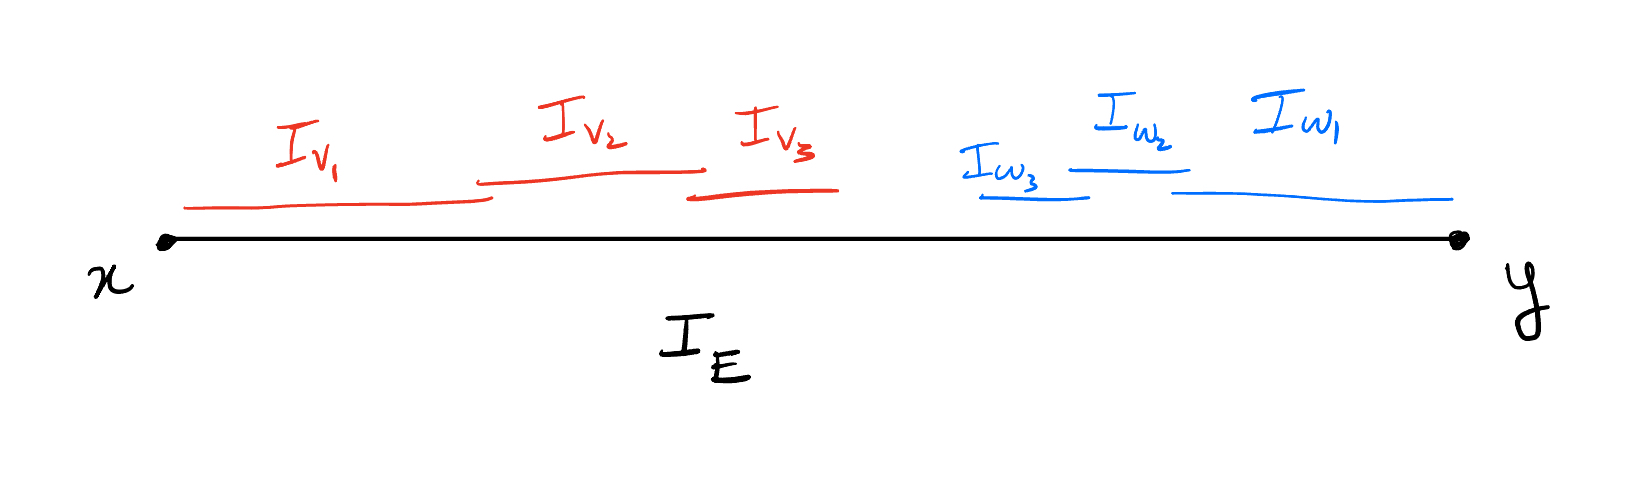
\includegraphics[scale=0.5]{images/subordering-example.png}
    \caption{Examples of $V_i \swarrow E$ and $E \searrow W_i$.}
    \label{fig:subordering-examples}
  \end{figure}

  In this example, all of the witnesses $V_i$ satisfy $V_i \swarrow E$, and all of the witnesses $W_i$ satisfy $E \searrow W_i$, but $d_E(\cC(V_i), x)$ need not be less than $9\mathbf{C}$ for $i=2$ or $i=3$, and similarly, $d_E(\cC(W_i), y)$ need not be less than $9 \mathbf{C}$ for $i=2$ or $i=3$.

  In fact, the above example illustrates that for witnesses $V$ that are not within distance $9 \mathbf{C}$ from one of the endpoints, the choice between assigning $V \swarrow E$ and $E \searrow V$ is ambiguous, which is what the property of being \emph{wide} tries to fix.
  The property of being \emph{wide} also tells when an active subsurface $V$ nested in a witness $E$ contributes to $E$: this happens when $V$ appears in the ``middle'' of the segment $[x,y]$.

  % \todo[inline]{Specify that this definition needs ISC witness families}

  \begin{definition}[Wide witness families]
    An insulated complete subordered witness family is wide if for each $V$ in the witness family, both of the following quantities are at most $\frac{N_V}{3}$.
    \begin{itemize}
    \item For $W$ a witness such that $W \swarrow V$, the quantity $\mathrm{diam}_V(x, \cC(W))$.
    \item For $W$ a witness such that $V \searrow W$, the quantity $\mathrm{diam}_V(y, \cC(W))$.
    \end{itemize}
  \end{definition}

  The idea behind a wide witness family is to create a buffer zone of length at least $\frac{N_V}{3}$ in the middle of the projection of the geodesic to $\cC(V)$ for any witness $V$ such that:
  \begin{itemize}
  \item If any subsurface $W$ is active to the left of the buffer zone, it contributes to a subsurface $Z$ such that $Z \swarrow V$.
  \item If any subsurface $W$ is active to the right of the buffer zone, it contributes to a subsurface $Z$ such that $V \searrow Z$.
  \item If a subsurface $W$ is active within the buffer zone, it contributes to $V$.
  \end{itemize}

  The upshot of defining wide, insulated, subordered, and complete witness families (which will be abbreviated to WISC witness families) is that it gives us a better idea the order in which progress is made in various active subsurfaces.
  If we were working with just the collection of active subsurfaces, the only time we can tell if a geodesic makes progress in a subsurface $V$ followed by the subsurface $W$ is when $V \pitchfork W$.
  When working with a WISC witness family, we can do that, but we can also make similar statements about pairs of nested witnesses $V \sqsubset W$, namely we can have either $V \swarrow W$ or $W \searrow V$.

  The following lemma asserts that WISC witness families exist, and their cardinality can be uniformly bounded.
  \begin{lemma}[Lemmas 7.29 and 7.30 from \cite{dowdall2023lattice}]
    Let $\os$ be surface, and $[x,y]$ a geodesic segment in $\teich(\os)$.
    Then there exists a WISC witness family $\Omega(x,y)$ for $[x,y]$.
    Furthermore, the cardinality of $\Omega(x,y)$ depends only on $\os$, and not the points $x$ and $y$.
  \end{lemma}
  \begin{rem}
    While the statements of Lemmas 7.29 and 7.30 in \textcite{dowdall2023lattice} are for orientable surfaces, they go through without any changes for non-orientable surfaces as well.
  \end{rem}

  We now get to the raison d'\^etre of witness families: turning points on the geodesic segment $[x,y]$ in $\teich(\os)$ into points in $\teich(V)$, where $V$ is a witness in $\Omega(x,y)$.
  We will do so by assigning to each point $w$ in a neighbourhood of $[x,y]$ a point $\wt{w}_Z$ in $\cC(Z)$ for all subsurfaces $Z$ contained in $V$, and then showing this assignment is consistent.
  Then the realization theorem (Theorem \ref{thm:consistency-realization}) will give us a point $\widehat{w}_V^{\Omega}$ in $\teich(V)$ which has the same projections in $\cC(Z)$ as the original point $W$.
  \begin{definition}[Projection tuple]
    \label{def:projection-tuple}
    Let $\Omega(x,y)$ be a WISC witness family for a Teichmüller geodesic $[x,y]$ in $\teich(\os)$.
    Let $w$ be a point in $\teich(\os)$ satisfying the following bound for every active subsurface $V$.
    \begin{align*}
      d_{V}(x, w) + d_{V}(w, y) \leq d_{V}(x, y) + 9 \mathbf{C}
    \end{align*}
    Then for any $U \in \Omega(x,y)$, the projection tuple $\wt{w}$ of $w$ is the point in $\prod_{Z \sqsubseteq U} \cC(Z)$ given by the following formula (where $\pi_Z$ is the usual projection map from $\teich(\os)$ to $\cC(Z)$).
    \begin{align*}
      \wt{w}_Z =
      \begin{cases}
        \pi_Z(y), & \text{if $Z \in \Upsilon(x,y)$ and $\colsup{Z}{\Omega} \swarrow U$} \\
        \pi_Z(x), & \text{if $Z \in \Upsilon(x,y)$ and $U \searrow \colsup{Z}{\Omega}$} \\
        \pi_Z(w), & \text{otherwise}
      \end{cases}
    \end{align*}
  \end{definition}

  Observe that this is different from the usual projection map from $\teich(\os)$ to $\cC(Z)$: for subsurfaces $Z$ that contribute to a witness nested in $U$, and consequently, $\colsup{Z}{\Omega} \swarrow U$ or $U \searrow \colsup{Z}{\Omega}$, we change the projection from $\pi_Z(w)$ to $\pi_Z(y)$ or $\pi_Z(x)$ respectively.
  % \todo[inline]{Motivate the reason for this modified projection map?}

  This new projection map, despite being a modification of the usual projection map, is still consistent.
  \begin{proposition}[Proposition 8.4 of \cite{dowdall2023lattice}]
    The projection tuple $\wt{w}_Z$ is $k$-consistent for some $k$ depending only on $\mathbf{C}$.
  \end{proposition}

  Using the above proposition, and the realization theorem for non-orientable surfaces (Theorem \ref{thm:consistency-realization}), we can turn a projection tuple into a point in $\teich(U)$, which \textcite{dowdall2023lattice} refer to as \emph{resolving a point $w$ in $\teich(U)$}.
  \begin{definition}[Resolution point]
    Let $[x,y]$ be a geodesic segment in $\teich(\os)$, and $\Omega(x,y)$ an associated WISC witness family.
    For $w \in \left\{ x, y \right\}$, and $U \in \Omega(x,y)$, we define $\widehat{w}_U^{\Omega}$ as follows.
    \begin{itemize}
    \item If $U$ is non-annular, then $\widehat{w}_U^{\Omega} \in \teich(U)$ is the thick point whose projections to $\cC(V)$ for $V \sqsubseteq U$ are coarsely equal to the projection tuple $\widehat{w}_U$ (which exists due to the Realization theorem (Theorem \ref{thm:consistency-realization})).
    \item If $U$ is annular, then $\wt{w}_U$ is an element of $\mathbb{Z}$, and we set $\widehat{w}_U^{\Omega}$ to be the point in $\mathbb{H}$ whose twist coordinate is $\wt{w}_U$, and whose length coordinate is $\displaystyle \frac{1}{\min\left( {\vept}, \ell_{\partial U}(w) \right)}$.
    \end{itemize}
  \end{definition}

  We can now define the complexity length associated to a witness family $\Omega$.

  \begin{definition}[Complexity of witness family]
    Let $[x, y]$ be a geodesic segment in $\teich(\os)$, and $\Omega$ an associated WISC witness family.
    The complexity $\mathfrak{L}_{\Omega}(x,y)$ of $\Omega$ is the following quantity.
    \begin{align*}
      \mathfrak{L}_{\Omega}(x,y) \coloneqq \sum_{U \in \Omega} \hNP^{\ast}(U) \cdot d_{\teich(U)}(\widehat{x}_{U}^{\Omega}, \widehat{y}_{U}^{\Omega})
    \end{align*}
    Here, $\hNP^{\ast}(U)$ is the net point growth entropy for $\teich(U)$ when $U$ is non-annular, and when $U$ is annular, $\hNP^{\ast}(U)$ is $1$ when both $\widehat{x}_{U}^{\Omega}$ and $\widehat{y}_{U}^{\Omega}$ are ${\vept}$-thick, and $2$ if not.
  \end{definition}

We now address why we used a modified version of the projection map in Definition \ref{def:projection-tuple} instead of the usual projection map to curve complexes, by revisiting Example \ref{ex:uninsulated}.
\begin{example}
  \label{ex:need-for-modified-projection}
  Let $\gamma$ be a pseudo-Anosov mapping class on $\os$, with large translation distance on $\cC(\os)$ and small projections elsewhere.
  Let $\delta$ be a reducible mapping class, which is psuedo-Anosov on a subsurface $V$, with large translation distance on $\cC(V)$ and small translation distance everywhere.
  Let $x$ be a point in $\teich(\os)$, and $y = \delta \gamma \delta^{-1} x$.
  We first verify that $\Upsilon(x,y) = \left\{ \os, V, \delta \gamma V \right\}$.
  To see this, we consider the following tuple of points $(x, \delta x, \delta \gamma x, \delta \gamma \delta^{-1}x)$.
  We claim that each of the points in the tuple lies coarsely on the geodesic $[x,y]$, and computing the projections of adjacent pairs of points in tuple, we get the following.
  \begin{itemize}
  \item[-] $[x, \delta x]$ has large projections on $\cC(V)$ and small projections on other curve complexes.
  \item[-] $[\delta x, \delta \gamma x]$ has large projections on the $\cC(\delta \os)$, which is the same as $\cC(\os)$, and small projections elsewhere.
  \item[-] $[\delta \gamma x, \delta \gamma \delta^{-1} x]$ has large projections on $\cC(\delta \gamma V)$, and small projections elsewhere.
  \end{itemize}
  Let $\Omega(x, y) = \Upsilon(x,y) = \left\{ \os, V, \delta \gamma V \right\}$.
  % \todo[inline]{Add more details about why $\delta \gamma V$ is the correct domain.}
  One can verify that this is a WISC witness family for $[x,y]$.
  Furthermore, we have that $V \swarrow \os$ and $\os \searrow \gamma V$.

  We now compute the resolution of the points $x$ and $y$ in $\teich(V)$, $\teich(\gamma V)$, and $\teich(\os)$.
  Observe that the geodesic $[x,y]$ almost immediately moves into a product region associated to $V$ at the beginning, leaves that product region at some point $w$ along the geodesic, and then enters the product region associated to $\gamma V$ at some point $z$, and then stays in that product region almost all the way up to the end.
  We will abuse notation slightly, and refer to $x$ and $w$ as points in $\teich(V)$, when we mean their projection via the product region map, and $z$ and $y$ will refer to points in $\teich(\gamma V)$
  Resolving points in $\teich(V)$ and $\teich(\gamma V)$ is easy, since there's no other witnesses nested in them, which means the projection tuple for those subsurfaces is the usual projection map.
  \begin{align*}
    \widehat{x}_V^{\Omega} &= x \\
    \widehat{y}_V^{\Omega} &= w \\
    \widehat{x}_{\gamma V}^{\Omega} &= z \\
    \widehat{y}_{\gamma V}^{\Omega} &= y \\
  \end{align*}
  To resolve points in $\teich(\os)$, we have to use our modified projection map, instead of the usual one.
  Doing so, the points $x$ and $y$ resolve in the following manner.
  \begin{align*}
    \widehat{x}_{\os}^{\Omega} = w \\
    \widehat{y}_{\os}^{\Omega} = z
  \end{align*}

  If we instead used the usual projection maps, $\widehat{x}_{\os}^{\Omega}$ would resolve to $x$, and $\widehat{y}_{\os}^{\Omega}$ would resolve to $y$.
  Consequently, we would not have the following estimate for complexity in terms of Teichmüller distance.
  \begin{align*}
    \mathfrak{L}_{\Omega}(x,y) &= \hNP^{\ast}(V) \cdot d_{\teich(V)}(x, w) + \hNP^{\ast}(\os) \cdot d_{\teich(\os)}(w, z) + \hNP^{\ast}(\gamma V) \cdot d_{\teich(\gamma V)}(z, y) \\
    &< \hNP^{\ast}(\os) \cdot d_{\teich(\os)}(x, y)
  \end{align*}
\end{example}

Constructing the resolution points $\widehat{x}_V^{\Omega}$ and $\widehat{x}_V^{\Omega}$ via the Realization theorem does not provide us very good bounds for $d_{\teich(V)}(\widehat{x}_V^{\Omega}, \widehat{x}_V^{\Omega})$.
At best, we accrue multiplicative and additive errors if we use Rafi's distance formula to estimate this distance from the curve complex distances.
For our applications however, the most we can tolerate is additive error.
To do this, we will need to refine to notion of active interval for a subsurface to something more useful for the estimate: the \emph{contribution set} $\mathcal{A}_V^{\Omega}$ of a witness $V$.
We first define two intermediate collections of subintervals of a geodesic segment $[x,y]$.
\begin{align*}
  M(V) &\coloneqq \bigcup \left\{ \mathcal{I}_W^{{\vept}} \mid \text{$W \in \Omega$ with $W \sqsubset V$ }  \right\} \\
  C(V) &\coloneqq \bigcup \left\{ \mathcal{I}_Z^{{\vept}} \mid \text{$Z$ contributes to $V$} \right\}
\end{align*}

\begin{definition}[Contribution set]
  For a witness $V \in \Omega$, the contribution set $\mathcal{A}_V^{\Omega}$ is a subset of the geodesic segment $[x,y]$ defined in the following manner.
  \begin{align*}
    \mathcal{A}_V^{\Omega} \coloneqq \left( \mathcal{I}_V^{\vept} \setminus M(V) \right) \cup C(V)
  \end{align*}
\end{definition}
\begin{rem}
  The reason we remove $M(V)$ and then later add $C(V)$ again is because it is possible for several different subsurfaces to be active at the same time: orthogonal subsurfaces for instance.
  One can have $V$ and $W$ as witnesses, with $W \sqsubset V$, and $Z \sqsubset V$ an active subsurface but not a witness, such that $W \perp Z$ with $\mathcal{I}_W^{\vept}$ and $\mathcal{I}_Z^{\vept}$ overlapping.
  In that case, removing $M(V)$ would also remove part of $\mathcal{I}_Z^{\vept}$, and adding back $C(V)$ would add back the deleted portion.
\end{rem}

The following theorem estimates $d_{\teich(V)}(\widehat{x}_V^{\Omega}, \widehat{y}_V^{\Omega})$ using $\mathcal{A}_V^{\Omega}$.
\begin{theorem}[Theorem 9.4 of \cite{dowdall2023lattice}]
  \label{thm:contribution-set-resolution-distance}
  There exists a uniform constant $C$ such that the following bound holds for any $x$, $y$, and witness $V$.
  \begin{align*}
d_{\teich(V)}(\widehat{x}_V^{\Omega}, \widehat{y}_V^{\Omega}) \leq \int_x^y \mathbbm{1}_{\mathcal{A}_V^{\Omega}} + C
  \end{align*}
\end{theorem}

Contribution sets help us make precise the notion of ``overcounting'' when multiple product regions are active at the same time.
More precisely, when a segment of $[x,y]$ is a part of two or more contribution sets, that segment shows up multiple times when computing $\mathfrak{L}_{\Omega}(x,y)$, thanks to Theorem \ref{thm:contribution-set-resolution-distance}.
If the overlapping segment is sufficiently long, one could even end up having $\mathfrak{L}_{\Omega}(x,y) > \hNP^\ast(\os) \cdot d_{\teich(\os)}(x, y)$, which as we will see, leads to a worse count for net points than the usual methods.
This phenomenon of contribution sets overlapping is called \emph{badness}, and while we will not be able to eliminate it entirely, we will be able to minimize it.

\begin{definition}[Bad set]
  We say a point $p$ in $\mathcal{A}_V^{\Omega}$ is bad if there exists some other witness $W$ such that $p$ also belongs in $\mathcal{A}_W^{\Omega}$.
  The bad set $\mathcal{B}_V^{\Omega}$ denotes the set of all bad points in $\mathcal{A}_V^{\Omega}$, and $\left| \mathcal{B}_V^{\Omega} \right|$ denotes the total length of this set, when we think of $\mathcal{B}_V^{\Omega}$ as a subset of the geodesic segment $[x,y]$.
\end{definition}

For our applications, we won't need to eliminate badness entirely, or even bound the length of the bad set uniformly: it will suffice to show that the length of the bad set is a very small multiple of $d_{\teich(\os)}(x,y)$.

\begin{definition}[Admissible and limited]
  A witness family $\Omega$ associated to a geodesic segment $[x,y]$ is said to be:
  \begin{itemize}
  \item \emph{admissible} if $\displaystyle \left| \mathcal{B}_V^{\Omega} \right| \leq \frac{d_{\teich(\os)}(x,y)}{K_V \mathbf{C}}$, for all $V \in \Omega$, and some constants $K_V$ that only depend on the topological type of $V$.
  \item \emph{limited} if $\left| \Omega \right|$ is uniformly bounded, independent of $x$ and $y$.
  \end{itemize}
\end{definition}
\begin{rem}
  Our definition of limited is a weaker version of Definition 10.7 from \textcite{dowdall2023lattice}, but since we don't need to stronger version, we present this version instead.
\end{rem}

\textcite{dowdall2023lattice} prove that WISC witness families that are admissible and limited exist. They call these witness families WISCAL witness families.

\begin{proposition}[Section 10.3 of \cite{dowdall2023lattice}]
  For all $[x,y]$, there exists an associated WISC witness family that is also admissible and limited.
\end{proposition}

For WISCAL witness families, the following result relating complexity and Teichmüller distance follows easily from Theorem \ref{thm:contribution-set-resolution-distance} and the definition of admissible.

\begin{proposition}
  \label{prop:complexity-length-inequality}
  If $\Omega$ is a WISCAL witness family associated to $[x,y]$, then the following inequality holds.
  \begin{align*}
    \mathfrak{L}_{\Omega}(x,y) \leq \left( \hNP(\os) + \frac{K}{\mathbf{C}} \right) d_{\teich(\os)}(x, y) + K \mathbf{C}
  \end{align*}
  Here, $K$ is some uniform constant depending only on $\os$.
\end{proposition}

% For triples of points that do not backtrack, there exists a version of the above inequality similar to a reverse triangle inequality.

% \begin{definition}[$\theta$-aligned]
%   A triple of points $(x,y,z)$ in $\teich(\os)$ is said to be $\theta$-aligned if the following inequality holds for all subsurfaces $V$.
%   \begin{align*}
%     d_V(x, y) + d_V(y, z) \leq d_V(x, z) + \theta
%   \end{align*}
% \end{definition}

% \begin{theorem}[Theorem 11.2 of \cite{dowdall2023lattice}]
%   If $(x, y, z)$ is a $\mathbf{C}$-aligned triple in $\teich(\os)$, and $\Omega_1$ is a WISCAL witness family for $[x,y]$, and $\Omega_2$ a WISCAL witness family for $[y,z]$, then the following inequality holds.
%   \begin{align*}
%     \mathfrak{L}_{\Omega_1}(x, y) + \mathfrak{L}_{\Omega_2}(y, z) \leq \left( \hNP(\os) + \frac{K}{\mathbf{C}} \right) d_{\teich(\os)}(x,z) + K \mathbf{C}
%   \end{align*}
%   Here, $K$ is some uniform constant depending only on $\os$.
% \end{theorem}

We now define complexity length, which follows from the definition of the complexity of a witness family.

\begin{definition}[Complexity length]
  \label{defn:complexity-length}
  For a pair of points $x$ and $y$ in $\teich(\os)$, the complexity length $\mathfrak{L}(x,y)$ is defined to be the following.
  \begin{align*}
    \mathfrak{L}(x,y) \coloneqq \inf_{\Omega} \mathfrak{L}_{\Omega}(x,y)
  \end{align*}
  Here, we take the infimum over all WISCAL witness families for $[x,y]$.
\end{definition}

With the machinery of complexity length set up, it is now possible to count net points with respect to complexity length.

\begin{theorem}[Theorem 12.1 of \cite{dowdall2023lattice}]
  \label{thm:counting-with-complexity}
  For any large enough $\mathbf{C} > 0$, and any $\veperr > 0$, there exists an polynomial function $p(r)$, and $r > 0$ large enough such that the following bound holds for net points in $\teich(\os)$.
  \begin{align*}
    \# \left( y \in \net \mid \mathfrak{L}(x,y) \leq r \right) \leq p(r) \cdot \exp\left( (1+\veperr)r \right)
  \end{align*}
\end{theorem}
%\todo[inline]{Make sure we're using consistent notation for net.}

\begin{rem}
  The above theorem is a slightly weaker version of the theorem that appears in \textcite{dowdall2023lattice}: their version does not have the $\veperr$.
  The reason we have the weaker version is that in the proof of their theorem, they count the number of net points in $\teich(V)$ in a ball of radius $R$, where $V$ is a witness, using Theorem \ref{thm:abem}, which gives them that the number of net points is equal, up to multiplicative error, to $\exp(\hNP(U) R)$.
  Since Theorem \ref{thm:abem} only holds orientable surfaces, and we want to state our results for non-orientable surfaces as well, we will need to use a weaker counting result to count net points in $\teich(V)$, namely the following bound, which holds for any $\vepent > 0$ and large enough $R$.
  \begin{align*}
    \#\left( y \in \net \mid d_{\teich(V)}(x, y) \leq R \right) \leq \exp\left( (\hNP(V) + \vepent ) R \right)
  \end{align*}
\end{rem}

We sketch out a proof of Theorem \ref{thm:counting-with-complexity} below: the proof proceeds identically to the proof in \textcite{dowdall2023lattice}, except at one point, where we plug in our weaker bound for net points in $\teich(V)$ for witnesses $V$.

\begin{proof}[Sketch of proof for Theorem \ref{thm:counting-with-complexity}]
  For each $y \in \net$ such that $\mathfrak{L}(x,y) \leq r$, we have a WISCAL witness family $\Omega$ such that $\mathfrak{L}_{\Omega}(x,y) \leq r$.
  We can turn that witness family into a graph in the following manner.
  \begin{itemize}
  \item Add a vertex for every witness $V \in \Omega$.
  \item Label the vertex associated with $V$ with the tuple $(\hNP^{\ast}(V), \lfloor d_{\teich(V)}(\widehat{x}_{V}^{\Omega}, \widehat{y}_{V}^{\Omega}) \rfloor)$.
  \item If we have a pair of witnesses $V \swarrow W$, we join the vertices associated to them with a directed edge labeled ``SW'': $V \xrightarrow{SW} W$.
  \item If we have a pair of witnesses $W \searrow V$, we join the vertices associated to them with a directed edge labeled ``SE'': $W \xrightarrow{SE} V$.
  \item If we have a pair of witnesses $W \pitchfork V$, with $W \lessdot V$, we join the vertices associated to them with a directed edge labelled ``P'': $W \xrightarrow{P} V$.
  \end{itemize}

  We first count how many distinct possibilities are there for such labeled graphs that correspond to $y$ for which $\mathfrak{L}(x,y) \leq r$.
  Since the cardinality of a WISCAL family is uniformly bounded, there are at most $k$ many vertices, for some constant $k$.
  As for the labels on the vertices, there are at most $\frac{r}{\hNP^{\ast}(V)}$ possibilities for a label on vertex which corresponds to a subsurface which is homeomorphic to $V$.
  From this, we conclude that there are at most $p(r)$ possibilities for the combinatorial type of the graph, where $p(r)$ is a polynomial in $r$.

  It will suffice to compute how many distinct net points give rise to witness families whose graph is of a given type.
  To do so, we consider \emph{initial subsets} of the graph, i.e. a subset $\mathcal{W}$ of the vertices $\mathcal{V}$ of the graph such that there is no directed edge from $\mathcal{V} \setminus \mathcal{W}$ to $\mathcal{W}$.

  Given an initial subset $\mathcal{W}$ of the graph, we construct points $y$ such that the witness family associated to $[x,y]$ has the combinatorial type $\mathcal{W}$.
  We then consider an enlargement of $\mathcal{W}$ by one-additional vertex $v$, such that the enlargement is still an initial subset.
  \begin{claim*}
    The entire graph $\mathcal{V}$ can be built up from such one-step enlargements.
  \end{claim*}

  We then count the number of net points whose associated witness families have the combinatorial type $\mathcal{W} \cup \left\{ v \right\}$, after we fix one witness family associated to $\mathcal{W}$.
  More concretely, let $w$ be a point such that the combinatorial type of the witness family associated to $[x,w]$ is $\mathcal{W}$.
  Suppose now that we add a vertex $(h, r_0)$ to the graph $\mathcal{W}$.
  To extend $\Omega(x,w)$ so that its combinatorial type is $\mathcal{W} \cup \left\{ (h, r_0) \right\}$, we need to add a witness $U$ whose net point entropy is $h$, and travel for distance $r_0$ in the Teichmüller space of $U$.
  There are only finitely many choices for such subsurfaces $U$ (because their boundary curves must get short near $w$), and once we've made a choice of $U$, we have a choice $\exp\left( (\hNP(V) + \vepent) r_0 \right)$ points.

  Multiplying out the counts for each vertex added, we get the following estimate for the cardinality associated to each combinatorial type.
  \begin{align*}
    \#\left( y \mid \text{$\Omega(x,y)$ has combinatorial type $\mathcal{V}$} \right) &= \sum_{(h, s) \in \mathcal{V}} \exp\left( (h + \vepent)s \right) \\
    &\leq \exp\left( (1 + \veperr)r \right)
  \end{align*}
  We get the second inequality by picking $\vepent$ small enough, and observing that $\sum hs = r$.
\end{proof}

\subsection{Linear gap for bad points}
\label{sec:linear-gap-bad}

In this subsection, we will prove our main result involving complexity length: on the complexity length of bad points.

\begin{theorem}
  \label{thm:linear-gap}
  Suppose that for all proper subsurfaces $V$ of $\os$, the following inequality holds.
  \begin{align*}
    \hNP(V) < \hNP(\os)
  \end{align*}
  Then for any $\vepb > 0$, there exists $c > 0$, and $R$ large enough, such that for any bad point $y$, i.e. a point in $\net_b(p, R, \vepb)$, the following upper bound holds for the complexity length between $p$ and $y$.
  \begin{align*}
    \mathfrak{L}(p, y) \leq \hNP(\os) (1 - c) R
  \end{align*}
\end{theorem}

\begin{proof}


Let $\Omega$ be a WISCAL witness family for $[p, y]$: the proof of Theorem \ref{thm:linear-gap} splits into two cases depending on whether the surface $\os$ is a witness in $\Omega$ or not.

The former case is harder, so we deal with that first.
% \begin{lemma}
%   The triple $(p, \widehat{y}_{\os}^{\Omega}, y)$ is $\theta$-aligned, for some constant $\theta$ independent of $R$ and $y$.
% \end{lemma}

% \begin{proof}
%   Recall that we define $\widehat{y}_{\os}^{\Omega}$ by specifying its coordinates in the curve complex of a subsurface $V$ according to the following rule.
%   \begin{itemize}
%   \item $\pi_V(y)$ if $\overline{V} \swarrow \os$.
%   \item $\pi_V(p)$ if $\os \searrow \overline{V}$.
%   \item $\pi_V(y)$ otherwise.
%   \end{itemize}
%   In all of these cases, the resulting triple in $\cC(V)$ looks like $(p,p,y)$ or $(p,y,y)$, which are trivially $\theta$-aligned for some uniform constant $\theta$.
% \end{proof}

We consider the triple of points $(p, \widehat{y}_{\os}^{\Omega}, y)$, and first estimate $\mathfrak{L}(p, \widehat{y}_{\os}^{\Omega})$.
% Observe that from the way we have defined $\widehat{y}_{\os}^{\Omega}$, it's within a bounded distance of the point $q$ on $[p,y]$ which is the last point on $[p, y]$ which stays in the thick part.

% By hypothesis of $y$ being a bad point, we have the following bounds on Teichmüller distance.
% \begin{align*}
%   % d_{\teich(\os)}(q, y) &> \vepb R \\
%   d_{\teich(\os)}(p, q) &\leq (1-\vepb) R
% \end{align*}
% Since $\widehat{y}_{\os}^{\Omega}$ is within bounded distance of $q$, we get similar bounds for $\widehat{y}_{\os}^{\Omega}$, with an additional constant $J$.
% \begin{align}
%   \label{eq:eq1}
%   % d_{\teich(\os)}(\widehat{y}_{\os}^{\Omega}, y) &> \vepb R - J \\
%   d_{\teich(\os)}(p, \widehat{y}_{\os}^{\Omega}) &\leq (1-\vepb) R + J
% \end{align}
By applying Proposition \ref{prop:complexity-length-inequality}, we get a bound for $\mathfrak{L}(p, \widehat{y}_{\os}^{\Omega})$.
\begin{align}
  \label{eq:eq2}
  \mathfrak{L}(p, \widehat{y}_{\os}^{\Omega}) \leq \left( \hNP(\os) + \frac{K}{\mathbf{C}} \right) (d_{\teich(\os)}(p, \widehat{y}_{\os}^{\Omega})) + K \mathbf{C}
\end{align}

We next estimate $\mathfrak{L}(\widehat{y}_{\os}^{\Omega}, y)$: we claim that there exists a WISCAL witness family $\Omega^{\prime}$ for $[\widehat{y}_{\os}^{\Omega}, y]$ that does not have $\os$ as a witness.
Indeed, we can construct this witness family from $\Omega$: take all the witnesses $V$ such that $\os \searrow V$.

Since the witness family $\Omega^{\prime}$ does not have $\os$ as a witness, we can do better than Proposition \ref{prop:complexity-length-inequality} when estimating $\mathfrak{L}(\widehat{y}_{\os}^{\Omega}, y)$.
We have from our hypothesis that $\hNP(\os) > \hNP(V)$, there exists a constant $h$ such that $h < \hNP(\os)$ but $h > \hNP(V)$.
Using Theorem \ref{thm:contribution-set-resolution-distance}, we get the following estimate for $\mathfrak{L}(\widehat{y}_{\os}^{\Omega}, y)$.
\begin{align}
  \label{eq:eq3p}
\mathfrak{L}(\widehat{y}_{\os}^{\Omega}, y) \leq \left( h + \frac{K}{\mathbf{C}} \right) d_{\teich(\os)}(\widehat{y}_{\os}^{\Omega}, y) + K \mathbf{C}
\end{align}

From the triangle inequality for complexity length, we also have the following
\begin{align}
  \label{eq:eq4}
  \mathfrak{L}(p, y) \leq \mathfrak{L}(p, \widehat{y}_{\os}^{\Omega}) + \mathfrak{L}(\widehat{y}_{\os}^{\Omega}, y)
\end{align}
We plug in \eqref{eq:eq2} and \eqref{eq:eq3p} into \eqref{eq:eq4}.
\begin{align*}
  \mathfrak{L}(p, y) &\leq \left( \hNP(\os) + \frac{K}{\mathbf{C}} \right) (d_{\teich(\os)}(p, \widehat{y}_{\os}^{\Omega})) + \left( h + \frac{K}{\mathbf{C}} \right) d_{\teich(\os)}(\widehat{y}_{\os}^{\Omega}, y) +  2K \mathbf{C} \\
                     &= \left( \hNP(\os) + \frac{K}{\mathbf{C}} \right) (d_{\teich(\os)}(p, \widehat{y}_{\os}^{\Omega}) + d_{\teich(\os)}(\widehat{y}_{\os}^{\Omega}, y)) \\
                     &- \left( \hNP(\os) - h \right) d_{\teich(\os)}(\widehat{y}_{\os}^{\Omega}, y) \\
  &+  2K \mathbf{C}
\end{align*}

Since $\widehat{y}_{\os}^\Omega$ is within a bounded distance of a point $q$ on $[p, y]$, we have $d_{\teich(\os)}(p, \widehat{y}_{\os}^{\Omega}) + d_{\teich(\os)}(\widehat{y}_{\os}^{\Omega}, y) \leq R + J$, for some constant $J$.
Furthermore, $d_{\teich(\os)}(\widehat{y}_{\os}^{\Omega}, y) \geq \vepb R$, by the hypothesis of $y$ being a bad point.
This simplifies the expression for $\mathfrak{L}(x,y)$.
\begin{align*}
  \mathfrak{L}(x,y) &\leq \left( \hNP(\os) + \frac{K}{\mathbf{C}} \right) R - (\hNP(\os) - h)(\vepb) R + 2K \mathbf{C} \\
  &= R \left( \hNP(\os) - d + \frac{K}{\mathbf{C}} \right) + 2K\mathbf{C}
\end{align*}
Here, $d = \vepb \left( \hNP(\os) - h \right)$, which is a positive constant, since $\hNP(\os) > h$.
By picking $\mathbf{C}$ and $R$ large enough, we get the statement of the theorem, which proves the result in the first case of $\os$ being in the witness family.

When $\os$ is not in the witness family, we set $\widehat{y}_{\os}^{\Omega} = p$, and the rest of the proof follows identically.
\end{proof}
\appendix

\section{Geometry of $\teich(\no_g)$}
\label{sec:geom-of-teich}

In this section, we prove some standard results about the geometry of Teichmüller spaces of non-orientable surfaces that we use in Section \ref{sec:line-gap-compl}.
We do so by lifting the hyperbolic structures and markings on the non-orientable surfaces to their double covers, which give us points in the Teichmüller space and curve complex of the double cover.

The fact that these lifts are well-defined and respect the metric properties are encapsulated in the following two theorems.

\begin{theorem}[Isometric embedding of Teichmüller spaces (Theorem 2.1 of \cite{limitsetkhan})]
  \label{thm:i-embedding-teich-space}
  The map $i : \teich(\no_g) \to \teich(\os_{g-1})$ given by lifting the hyperbolic structure and marking from $\no_g$ to $\os_{g-1}$ is an isometric embedding.
  Furthermore, the image of $\teich(\no_g)$ in $\teich(\os_{g-1})$ is the subset of $\teich(\os_{g-1})$ is fixed by $\iota^{\ast}$, where $\iota^{\ast}$ is the map induced by the orientation reversing deck transformation $\iota$ on $\os_{g-1}$.
\end{theorem}

\begin{theorem}[Quasi isometric embedding of curve complexes (Lemma 6.3 from \cite{masur2013geometry})]
  \label{thm:qi-embedding-curve-complex}
  The map $\cC(\no_g) \to \cC(\os_{g-1})$ obtained by lifting curves in $\no_g$ to $\os_{g-1}$ is a quasi-isometric embedding.
\end{theorem}

We will use the above two theorems, along with Lemma \ref{lem:lifting-subsurfaces}, to reduce statements about the geometry of $\teich(\no_g)$ to statements about the geometry of $\teich(\os_{g-1})$.
However, we postpone the statement and the proof of Lemma \ref{lem:lifting-subsurfaces} until Section \ref{sec:dist-form-teichm}, since it's not required for Section \ref{sec:minskys-prod-regi}.

We set up some notation for this section.
\begin{itemize}
\item[-] $d(x,y)$ and $d(\wt{x}, \wt{y})$: Given points $x$ and $y$ in $\teich(\no_g)$, $d(x, y)$ is the distance in Teichmüller metric between them, and $d(\wt{x}, \wt{y})$ is the distance in $\teich(\os_{g-1})$ between their images, $\wt{x}$ and $\wt{y}$.
\item[-] $\pi_V(\mu_x)$ and $\pi_V(x)$: If $\mu_x$ is a marking/curve on a surface, the $\pi_V(\mu_x)$ denotes the subsurface projection to the subsurface $V$. If $x$ is a point in the Teichmüller space, the $\pi_V(x) = \pi_V(\mu_x)$, where $\mu_x$ is the Bers marking on $x$.
\item[-] $d_V(\mu_x, \mu_y)$ and $d_V(x, y)$: If $\mu_x$ and $\mu_y$ are markings/curves on a surface, and $V$ is a subsurface, then $d_V(\mu_x, \mu_y)$ refers to the curve complex distance between the subsurface projections of $\mu_x$ and $\mu_y$ in $\cC(V)$.
  When $x$ and $y$ are points in Teichmüller space, $d_V(x,y)$ refers to $d_V(\mu_x, \mu_y)$, where $\mu_x$ and $\mu_y$ are the Bers marking on $x$ and $y$.
\end{itemize}

\todo[inline]{Set up the notation, i.e. the various metrics floating around.}

\subsection{Minsky's product region theorem}
\label{sec:minskys-prod-regi}

In this section, we prove a version of Minsky's product region theorem \cite[Theorem 6.1]{1077244446} for non-orientable surfaces.

% Let $\gamma = \left\{ \gamma_1, \ldots, \gamma_j, \ldots, \gamma_k \right\}$ be a multicurve on a non-orientable surface $\no_g$, where for $i \leq j$, $\gamma_i$ is a two-sided curve, and for $i > j$, $\gamma_i$ is a one-sided curve.
% Let $X_\gamma$ denote the product $\teich(\no_g \setminus \gamma) \times \mathbb{H}_1 \times \cdots \times \mathbb{H}_j \times (\mathbb{R}_{>0})_{j+1} \times \cdots \times (\mathbb{R}_{>0})_k$.
% For any pants decomposition that contains $\gamma$, we get a map $\Pi$ from $\teich(\no_g)$ to $X_\gamma$, which is called the \emph{product region projection map}.
% \begin{definition}[Product region projection map]
%   The product region projection map $\Pi: \teich(\no_g) \to X_\gamma$ is defined in the following manner.
%   \begin{itemize}
%   \item The $\teich(\no_g \setminus \gamma)$-coordinate is obtained by pinching all the curves in $\gamma$ to get a punctured hyperbolic surface.
%   \item The $\mathbb{H}_i$-coordinate is $\left( t, \frac{1}{\ell} \right)$, where $t$ is the \emph{twist} of the two-sided curve $\gamma_i$, and $\ell$ is the hyperbolic length.
%   \item The $(\mathbb{R}_{>0})_i$ coordinate is $\frac{1}{\ell}$, where $\ell$ is the hyperbolic length of the one-sided curve $\gamma_i$.
%   \end{itemize}
% \end{definition}

% We define a metric on the product $X_\gamma$ as the supremum of the metrics on each of the components, where the metric on $\teich(\no_g \setminus \gamma)$ is the Teichmüller metric, the metric on the $\mathbb{H}_i$ components is the hyperbolic metric, and the metric on the $(\mathbb{R}_{>0})_i$ is given by $d(x,y) = \left| \log\left( \frac{x}{y}  \right) \right| $, i.e. the restriction of the hyperbolic metric in $\mathbb{H}$ to a vertical line.

% We will be interested in looking at the restriction of $\Pi$ to the thin region of Teichmüller space, denoted $\teich_{\gamma \leq \vept}(\no_g)$, which is the region where all curves in $\gamma$ have hyperbolic length at most $\vept$.

We recall the following objects that were defined in Section \ref{sec:weak-conv-syst}.

\begin{enumerate}[(i)]
\item The multicurve $\gamma$ on $\no_g$.
\item The metric space $X_\gamma$, and the projection map $\Pi$.
\item The thin region $\teich_{\gamma \leq \vept}(\no_g)$.
\end{enumerate}

\begin{theorem}[Product region theorem for non-orientable surfaces]
  \label{thm:prno}
  For any $c >0$, there exists a small enough $\vept > 0$, such that the restriction of $\Pi$ to $\teich_{\gamma \leq \vept}(\no_g)$ is an isometry with additive error at most $c$, i.e. the following holds for any $x$ and $y$ in $\teich_{\gamma \leq \vept}(\no_g)$.
  \begin{align*}
    \left| d(x, y) - d_{X_{\gamma}}(\Pi(x), \Pi(y)) \right| \leq c
  \end{align*}
\end{theorem}

\begin{proof}
  We will prove this result by reducing the distance calculation in $\teich(\no_g)$ to a distance calculation in $\teich(\os_{g-1})$, where $\os_{g-1}$ is the orientation double cover, and invoking the classical product region theorem in that setting.

  We begin the proof by constructing some points in $\teich(\os_{g-1})$ and a multicurve on $\os_{g-1}$.
  Recall that $\teich(\no_g)$ isometrically embeds inside $\teich(\os_{g-1})$: let $\wt{x}$ and $\wt{y}$ denote the points in $\teich(\os_{g-1})$ that are the images of $x$ and $y$ under the embedding.
  Let $\wt{\gamma}$ denote the lift of the multicurve $\gamma$: if $\gamma_i$ is a two-sided curve, it will have two disjoint lifts in the cover, and if $\gamma_i$ is a one-sided curve, it will have single lift in the double cover.
  We have that the region $\teich_{\wt{\gamma} \leq \vept}(\os_{g-1}) \subset \teich(\os_{g-1})$ intersects the image of $\teich(\no_g)$ at the image of $\teich_{\gamma \leq \vept}(\no_g) \subset \teich(\no_g)$.
  Let $\iota$ denote the orientation reversing deck transformation on $\os_{g-1}$ which corresponds to the covering map.

  \begin{claim*}
    Let $\Pi_k$ denote the projection map from $\teich(\no_g)$ to the $k$\textsuperscript{th} component of $X_\gamma$, and $\wt{\Pi_k}$ denote the projection map from $\teich(\os_{g-1})$ to the lift of the $k$\textsuperscript{th} component of $\gamma$ to $\os_{g-1}$.
    This map is an isometric embedding.
    \begin{align*}
      d(\Pi_k(x), \Pi_k(y)) = d(\wt{\Pi_k}(\wt{x}), \wt{\Pi_k}(\wt{y}))
    \end{align*}
  \end{claim*}
  % \todo[inline]{Explain this better. Maybe have a claim here.}

  \begin{proof}[Proof of claim]
  We need to verify the claim on the three kinds of components of $\gamma$.
  \begin{enumerate}[(i)]
  \item $\no_g \setminus \gamma$: The lift of $\no_g \setminus \gamma$ to $\os_{g-1}$ will have two components if $\no_g \setminus \gamma$ is orientable, which we call $S_1$ and $S_2$. Both $S_1$ and $S_2$ are homeomorphic to $\no_g \setminus \gamma$.
    If $\no_g \setminus \gamma$ is non-orientable, then its lift in $\os_{g-1}$ is the orientation double cover.

    In the first case, $\teich(\no_g \setminus \gamma)$ maps to the diagonal subspace in $\teich(S_1) \times \teich(S_2)$, and the metric on $\teich(S_1) \times \teich(S_2)$ is the $\sup$ metric.
    The space $\teich(\no_g)$ maps to the diagonal subspace because its image must be invariant under the map $\iota$, which isometrically swaps $S_1$ and $S_2$.
    This map is an isometric embedding, and thus for any points $x$ and $y$ in $\teich(\no_g \setminus \gamma)$, the distance between their images in $\teich(S_1) \times \teich(S_2)$ is the same as the distance in $\teich(\no_g \setminus \gamma)$.

    In the second case, we have that $\teich(\no_g \setminus \gamma)$ also isometrically embeds inside the Teichmüller space of its double cover, by Theorem \ref{thm:i-embedding-teich-space}, so the claim follows.
  \item $\gamma_i$ (for $\gamma_i$ two-sided): The lift of $\gamma_i$ in this case are two disjoint curves on $\os_{g-1}$, which are swapped by the deck transformation $\iota$.
    This means the $\mathbb{H}$-coordinate given by length and twist of $\gamma_i$ maps to the diagonal in $\mathbb{H} \times \mathbb{H}$, which correspond the length and twist around the two lifts.
    Since $\mathbb{H}$ mapped to the diagonal in $\mathbb{H} \times \mathbb{H}$ is an isometric embedding with $\sup$ metric, the claim follows in this case.
  \item $\gamma_i$ (for $\gamma_i$ one-sided): The lift of $\gamma_i$ in this case is a single curve $\wt{\gamma_i}$ on $\os_{g-1}$ which is left invariant by the deck transformation $\iota$.
    We will show that the twist coordinate around $\wt{\gamma_i}$ cannot be changed without leaving the image of $\teich(\no_g)$ in $\teich(\os_{g-1})$, i.e. any $\wt{x}$ and $\wt{y}$ have the same twist coordinate around $\wt{\gamma_i}$.
    Once we have established that, the claim will follow, since only the length coordinate of $\gamma_i$ can be changed, which corresponds to $\mathbb{R}_{>0}$.

    Suppose now that $x$ is a point in $\teich(\no_{g})$ and $\wt{x}$ the corresponding point in $\teich(\os_{g-1})$.
    Consider a pants decomposition on $\no_g$ that contains $\gamma_i$ as one of the curves. There is a unique one-sided curve $\kappa$ that intersects $\gamma_i$ and does not intersect any of the other pants curves.
    Let $\wt{\kappa}$ be the lift of $\kappa$ to $\os_{g-1}$: we will use this curve to measure twisting around $\wt{\gamma_i}$.
    Let $x^{\prime}$ be another point in $\teich(\os_{g-1})$ obtained by taking $\wt{x}$, and twisting by some amount around $\wt{\gamma_i}$, without changing the length of $\wt{\gamma_i}$.
    On $x^{\prime}$, the length of $\wt{\kappa}$ will be different from the length on $\wt{x}$.
    However, this means that $x^{\prime}$ is not contained in the image of $\teich(\no_g)$, since if it were, the length of $\wt{\kappa}$ would have to be the same, since that's the lift of the curve $\kappa$, whose length only depends on the length of $\gamma_i$.
  \end{enumerate}
  \end{proof}

  The following equality follows from the claim.
  \begin{align*}
    d_{X_{\wt{\gamma}}}(\Pi(\wt{x}), \Pi(\wt{y})) = d_{X_{{\gamma}}}(\Pi({x}), \Pi({y}))
  \end{align*}
  We also have that $\teich(\no_g)$ isometrically embeds into $\teich(\os_{g-1})$.
  \begin{align*}
    d(\wt{x}, \wt{y}) = d(x, y)
  \end{align*}
  And finally, have that the region $\teich_{\wt{\gamma} \leq \vept}(\os_{g-1}) \subset \teich(\os_{g-1})$ intersects the image of $\teich(\no_g)$ at the image of $\teich_{\gamma \leq \vept}(\no_g) \subset \teich(\no_g)$.
  Combining these three facts, and applying Minsky's product region theorem for orientable surfaces, the result follows.
\end{proof}

% {\color{red} Move the theorem in Section 3 to this section}

\subsection{Uniform bounds for the volume of a ball}
\label{sec:unif-bounds-volume}

Outline of section:
\begin{enumerate}[(i)]
\item Define the volume form $\nu_N$.
\item {\color{red} Prove a version of Lemma 3.1 for the Norbury volume form $\nu_N$ using the product region theorem.}
\end{enumerate}



\subsection{Teichmüller geodesics and geodesics in the curve complex}
\label{sec:dist-form-teichm}

In this section, we will deduce some standard results about Teichmüller geodesics and the corresponding curve complex geodesics for non-orientable surfaces by reducing to the orientable case.
The following lemma will be the main tool for the reduction to the orientable case.
\begin{lemma}
  \label{lem:lifting-subsurfaces}
  Let $[x, y]$ be a Teichmüller geodesics segment in $\teich(\no)$, where $\no$ is a non-orientable surface, and $[\wt{x}, \wt{y}]$ be its image in $\teich(\os)$, where $\os$ is the orientable double cover of $\no$.
  Let $V$ be a subsurface of $S$: then the following for $d_V(\wt{x}, \wt{y})$.
  \begin{enumerate}[(i)]
  \item If $V$ is the lift of a non-orientable subsurface $W$ in $\no$, then $d_V(\wt{x}, \wt{y}) \emul d_W(x, y)$.
  \item If $V$ is the lift of an orientable subsurface $W$ in $\no$, then $d_V(\wt{x}, \wt{y}) = d_{\iota(V)}(\wt{x}, \wt{y}) = d_W(x, y)$.
  \item If $V$ is not a lift of a subsurface in $\no$, then there exists a uniform constant $k_0$, independent of $x$, $y$, and $V$, such that $d_V(\wt{x}, \wt{y}) \leq k_0$.
  \end{enumerate}
\end{lemma}
\begin{proof}
  We deal with the proof in cases.
  \begin{enumerate}[(i)]
  \item If $V$ is the lift of an orientable surface, we have that the covering map restricted to $V$ is a homeomorphism, and the same holds for $\iota(V)$, so the result follows in this case as well.
  \item If $V$ is the lift of a non-orientable subsurface $W$, then by Theorem \ref{thm:qi-embedding-curve-complex}, we have that $\cC(W)$ quasi-isometrically embeds into $\cC(V)$, and the result follows.
  \item If $V$ is not a lift at all, that means $V$ and $\iota(V)$ are transverse subsurfaces.
    By the Behrstock inequality, there exists a $k_0$ such that the following holds.
    \begin{align}
      \label{ineq:min-of-equal}
      \min(d_V(\wt{x}, \wt{y}), d_{\iota(V)}(\wt{x}, \wt{y})) \leq k_0
    \end{align}
    Note that we also have that $\wt{x}$ and $\wt{y}$ are fixed by $\iota^{\ast}$, the induced map on $\teich(\os)$, which gives us the following.
    \begin{align*}
      d_{\iota(V)}(\wt{x}, \wt{y}) &= d_{V}(\iota^{\ast}(\wt{x}), \iota^{\ast}(\wt{y})) \\
                                   &= d_V(\wt{x}, \wt{y})
    \end{align*}
    This means that both the terms appearing in the $\min$ in \eqref{ineq:min-of-equal} are equal, which gives us the result.
  \end{enumerate}
\end{proof}

% \todo[inline]{Set up some context.}
We begin by proving the distance formula for points in Teichmüller space.
Let $x$ and $y$ be a pair of points in $\teich(\no_g)$, and let $\Gamma$ be the set of curves that are short on both $x$ and $y$, $\Gamma_x$ the set of curves that are only short on $x$, and $\Gamma_y$ the set of curves that are only short on $y$.
Let $\mu_x$ and $\mu_y$ be short markings on $x$ and $y$ respectively.
Let $\cC^+$ and $\cC^-$ denote the set of two-sided and one-sided curves on $\no_g$.
Finally, let $\left[ x \right]_k$ be the function which is $0$ for $x \leq k$, and identity for $x > k$.

\begin{theorem}[Distance formula]
  \label{thm:distance-formula}
  The distance between $x$ and $y$ in $\teich(\no_g)$ is given by the following formula.
  \begin{equation}
  \begin{aligned}
    d(x, y) &\emul \sum_{Y} \left[ d_Y(\mu_x, \mu_y) \right]_k + \sum_{\alpha \in \Gamma^c \cap \cC^+} \left[ \log(d_{\alpha}(\mu_x, \mu_y)) \right]_k \\
    &+ \max_{\alpha \in \Gamma \cap \cC^+} d_{\mathbb{H}_{\alpha}}(x, y) + \max_{\alpha \in \Gamma \cap \cC^-} d_{(\mathbb{R}_{>0})_{\alpha}}(x, y) \\
    &+ \max_{\alpha \in \Gamma_x} \log \frac{1}{\ell_x(\alpha)} + \max_{\alpha \in \Gamma_y} \log \frac{1}{\ell_y(\alpha)}
  \end{aligned}
  \label{eq:distance-formula-nonorient}
  \end{equation}
\end{theorem}
\begin{proof}
  Let $\wt{x}$ and $\wt{y}$ be the images of $x$ and $y$ in $\teich(\os_{g-1})$ under the isometric embedding map.
  Since $d(x,y) = d(\wt{x}, \wt{y})$, it will suffice to estimate $d(\wt{x}, \wt{y})$ using distances in the curve complexes.
  Let $\wt{\mu_x}$ and $\wt{\mu_y}$ be the lifts of $\mu_x$ and $\mu_y$.
  Both $\wt{\mu_x}$ and $\wt{\mu_y}$ are short markings on $\wt{x}$ and $\wt{y}$ respectively.
  We have by Rafi's distance formula \cite[Theorem 6.1]{rafi2007combinatorial}, the following estimate on $d(\wt{x}, \wt{y})$.
  \begin{equation}
  \begin{aligned}
    d(\wt{x}, \wt{y}) &\emul \sum_{Y} \left[ d_Y(\wt{\mu_x}, \wt{\mu_y}) \right]_k + \sum_{\alpha \in \wt{\Gamma}^c} \left[ \log(d_{\alpha}(\wt{\mu_x}, \wt{\mu_y})) \right]_k \\
    &+ \max_{\alpha \in \wt{\Gamma}} d_{\mathbb{H}_{\alpha}}(\wt{x}, \wt{y})\\
    &+ \max_{\alpha \in \wt{\Gamma_{\wt{x}}}} \log \frac{1}{\ell_{\wt{x}}(\alpha)} + \max_{\alpha \in \Gamma_{\wt{y}}} \log \frac{1}{\ell_{\wt{y}}(\alpha)}
  \end{aligned}
  \label{eq:distance-formula-orient}
  \end{equation}
  Here, $\wt{\Gamma}$, $\wt{\Gamma_{\wt{x}}}$, and $\wt{\Gamma_{\wt{y}}}$ are curves on $\wt{x}$ and $\wt{y}$ that are simultaneously short, short on $\wt{x}$ and not on $\wt{y}$, and short on $\wt{y}$ and not on $\wt{x}$ respectively.

 It will suffice to show that for a large enough choice of $k$, the right hand side of \eqref{eq:distance-formula-nonorient} is equal to the right hand side of \eqref{eq:distance-formula-orient}, up to an additive and multiplicative constant.
 We consider the first term in the right hand side of \eqref{eq:distance-formula-orient}, namely the sum over the non-annular subsurfaces $Y$.
 There are three possibilities for $Y$ in $\os_{g-1}$, which we deal with using Lemma \ref{lem:lifting-subsurfaces}.
 \begin{enumerate}[(i)]
 \item $Y$ is one component of a lift of an orientable subsurface $Z$ of $\no_g$: In this case we have $d_Y(\wt{\mu_x}, \wt{\mu_y}) = d_Z(\mu_x, \mu_y)$ (and the same equality with $Y$ replaced with $\iota(Y)$).
   Thus, for every term associated to an orientable non-annular subsurface $Z$ in \eqref{eq:distance-formula-nonorient}, we get two corresponding equal terms in \eqref{eq:distance-formula-orient}.
 \item $Y$ is the lift of a non-orientable subsurface $Z$ of $\no_g$: In this case, we have $d_Y(\wt{\mu_x}, \wt{\mu_y}) \emul d_Z(\mu_x, \mu_y)$.
 \item $Y$ is not a lift of a subsurface of $\no_g$: In this case, we have the following for some $k_0$.
   \begin{align*}
     d_Y(\wt{\mu_x}, \wt{\mu_y}) \leq k_0
   \end{align*}
   If we pick a threshold $k > k_0$, the subsurfaces $Y$ that do not arise from lifts will not contribute to the right hand side of \eqref{eq:distance-formula-orient}.
 \end{enumerate}
 % The analysis of the three possible types of non-annular subsurfaces $Y$ shows that the first terms on the right hand side of \eqref{eq:distance-formula-nonorient} and \eqref{eq:distance-formula-orient} are equal up to a multiplicative and additive constant, for $k > k_0$.

 We now do the same case analysis for annular subsurfaces: consider a curve $\alpha$ on $\os_{g-1}$ that is contained in $\Gamma^c$, i.e. it is not simultaneously short on $\wt{x}$ and $\wt{y}$. There are three possibilities for $\alpha$.
 \begin{enumerate}[(i)]
 \item $\alpha$ is one component of a lift of a two-sided curve $\gamma$ on $\no_g$: In this case, $\alpha$ and $\iota(\alpha)$ are disjoint, and the restriction of the covering map to these curves is a homeomorphism.
   We have $d_\alpha(\wt{\mu_x}, \wt{\mu_y}) = d_\gamma(\mu_x, \mu_y)$: consequently, for every term in $\Gamma^c \cap \cC^+$ in \eqref{eq:distance-formula-nonorient}, we have two equal terms in \eqref{eq:distance-formula-orient}.
 \item $\alpha$ is the lift of a one-sided curve on $\no_g$: In this case $\alpha = \iota(\alpha)$, but the transformation $\iota$ reverses orientation on the surface $\os_{g-1}$.
   That means $\wt(\mu_x)$ and $\wt{\mu_y}$ cannot have a relative twist between them along $\alpha$, because if they did, $\iota(\wt(\mu_x))$ and $\iota(\wt(\mu_y))$ would have the opposite twist.
   On the other hand $\wt{\mu_i} = \iota(\wt{\mu_i})$ for $i=x$ and $i=y$, which means the relative twist must be $0$.
   This proves that the $\alpha$ which are lifts of one-sided curves do not contribute to the second term of \eqref{eq:distance-formula-orient}.
 \item $\alpha$ is not a lift of a curve on $\no_g$: In this case $\alpha$ and $\iota(\alpha)$ intersect each other, and are not equal, which means they are transverse.
   We deal with this the same way we dealt with transverse non-annular subsurfaces, i.e. via the Behrstock inequality.
 \end{enumerate}
 This case analysis proves that the second terms on the right hand side of \eqref{eq:distance-formula-nonorient} and \eqref{eq:distance-formula-orient} are equal, up to an additive and multiplicative constant.

We now deal with the last three terms of \eqref{eq:distance-formula-orient}.
These terms deal with short curves on $x$ or $y$: we claim that the short curves must be lifts of either one-sided or two-sided curves in $\no_g$.
Suppose a curve $\alpha$ is short and not a lift. Then $\alpha$ has positive intersection number with $\iota(\alpha)$, but since $\iota$ is an isometry, $\iota(\alpha)$ must also be short.
For a sufficiently small threshold for what we call short, we can't have a short curve intersecting another short curve, which proves the claim that all the short curves arise as lifts.

Since the curves in $\wt{\Gamma}$ are all lifts, the third term of \eqref{eq:distance-formula-orient} can be split up into two terms: the lifts of the two-sided and one-sided curves.
For the two-sided curves, the distance calculation involves both the length and twist coordinate, and for the one-sided curves, only the length coordinate is involved.
This follows from Theorem \ref{thm:prno}.

Finally, the last two terms in \eqref{eq:distance-formula-orient} are the same as the last two terms of \eqref{eq:distance-formula-nonorient}, up to an additive error of $(6g) \cdot \log(2)$, since the lift of a short curve can double its length, and there are no more than $6g$ short curves.

We have shown that the right hand sides of \eqref{eq:distance-formula-nonorient} and \eqref{eq:distance-formula-orient} are equal, up to a multiplicative and additive constant, which proves the result.
\end{proof}

We now verify that Teichmüller geodesics can be broken up into \emph{active intervals associated to subsurfaces}, which are subintervals of the geodesic associated to each subsurface $V$, along which the projection to $V$ is large, and outside of which, the projection is bounded.
% To build up the machinery of complexity length, we will also need a description of the Teichmüller geodesic segments.
% Let $[x, y]$ be a Teichmüller geodesic segment between $x$ and $y$ in $\teich(\no_g)$.
The following lemma  of \textcite[Lemma 3.26]{dowdall2023lattice} (which itself is a generalization of \textcite[Proposition 3.7]{rafi2007combinatorial}) describes the subsegments of $[x,y]$ along which the geodesic makes progress in the curve complex of a subsurface.

\begin{proposition}
  \label{thm:active-intervals}
  For each sufficiently small $\vept > 0$, there exists $0 < {\vept}^{\prime} < \vept$ and $M_{\vept} \geq 0$ such that for any subsurface $V \sqsubset S$, there's a (possibly empty) connected interval $\mathcal{I}_V^{\vept} \subset [x,y]$ such that the following five conditions hold.
  \begin{enumerate}[(i)]
  \item If $d_V(x, y) \geq M_{\vept}$, then $\mathcal{I}_V^{{\vept}}$ is a non-empty subinterval of $[x,y]$.
  \item $\ell_\alpha(z) < {\vept}$ for all $z \in \mathcal{I}_V^{{\vept}}$ and $\alpha \in \partial V$.
  \item For all $z \in [x,y] \setminus \mathcal{I}_V^{{\vept}}$, some component $\alpha$ of $\partial V$ has $\ell_\alpha(z) > {\vept}^{\prime}$.
  \item $d_V(w, z) \leq M_{\vept}$ for every subinterval $[w,z] \subset [x,y]$ if $[w,z] \cap \mathcal{I}_V^{\vept} = \varnothing$.
  \item For a pair of traverse subsurfaces $U$ and $V$, $\mathcal{I}_U^{\vept} \cap \mathcal{I}_V^{\vept} = \varnothing$.
  \end{enumerate}
\end{proposition}

\begin{proof}[Proof of Theorem \ref{thm:active-intervals} for non-orientable surfaces]
  Let $\no$ be the non-orientable surface, and $\os$ its double cover.
  We consider the image $[\wt{x}, \wt{y}]$ of the geodesic $[x,y]$ in $\teich(\os)$.
  We know that the result holds for $[\wt{x}, \wt{y}]$, although with ${\vept}^{\prime}$ replaced with $\frac{{\vept}^{\prime}}{2}$, since lifting can double the lengths of some curves.

  The main fact we need to verify is that the only subsurfaces $V$ that have non-empty $\mathcal{I}_V^{\vept}$ come from lifts.
  If $V$ is a subsurface of $\os$ that is not a lift, we use case (iii) of Lemma \ref{lem:lifting-subsurfaces} to conclude that $d_V(x, y) \leq k_0$ for some fixed constant $k_0$.
  Picking $M_{\vept} > k_0$ guarantees that the only subsurfaces for which $\mathcal{I}_V^{\vept}$ is non-empty arise from lifts, which proves the result for non-orientable surfaces.
\end{proof}

Finally, we show that the consistency and the realization results (\textcite{behrstock2012geometry}) hold for Teichmüller spaces of non-orientable surfaces as well.
We begin by recalling the definition of consistency.

\begin{definition}[Consistency]
  For a connected surface $S$, and a parameter $\theta \geq 1$, we say a tuple $(z_V) \in \prod_{V \sqsubset S} \cC(V)$ is $\theta$-consistent if the following two conditions holds for all pairs of subsurfaces $U$ and $V$.
  \begin{enumerate}[(i)]
  \item If $U \pitchfork V$, then
    \begin{align*}
      \min(d_U(z_U, \partial V), d_V(z_V, \partial U)) \leq \theta
    \end{align*}
  \item If $U \sqsubset V$, then
    \begin{align*}
      \min(d_U(z_U, \pi_U(z_V)), d_V(z_V, \partial U)) \leq \theta
    \end{align*}
  \end{enumerate}
\end{definition}
\todo[inline]{Make sure I use the transversality notation consistently.}

The following theorem (\textcite[Theorem 4.3]{behrstock2012geometry}) states that the projection from Teichmüller space to the curve complexes of all the subsurfaces is coarsely surjective onto the set of consistent tuples.

\begin{theorem}[Consistency and realization]
  \label{thm:consistency-realization}
  There is a constant $K \geq 1$, and function $\mathfrak{C}: \mathbb{R}_+ \to \mathbb{R}_+$ such that the following holds for any surface $S$.
  \begin{itemize}
  \item (Consistency) For every $x \in \teich(S)$, the projection tuple $(\pi_V(x))_{V \sqsubset S}$ is $K$-consistent.
  \item (Realization) For every $\theta$-consistent tuple $(z_V)_{V \sqsubset S}$, there exists a point $z \in \teich(S)$ such that $d_V(\pi_V(z), z_V) \leq \mathfrak{C}(\theta)$ for all $V$.
  \end{itemize}
\end{theorem}
\begin{proof}[Proof sketch of Theorem \ref{thm:consistency-realization} for non-orientable surfaces]
    We first show that the projection map is consistent, and then show consistent tuples lie coarsely in the image of the projection map.
  \begin{itemize}
  \item (Consistency) We map $x$ to $\wt{x}$ in the Teichmüller space of the double cover $\wt{S}$.
    By applying the theorem for orientable surfaces, we have the $(\pi_{W}(\wt{x}))_{W \sqsubset \wt{S}}$, and we restrict to the subsurfaces in the tuple which arise as lifts.
    These points lie in the image of the quasi-isometric embedding map from Theorem \ref{thm:qi-embedding-curve-complex}, which means consistency also holds for the tuples in $S$.
  \item (Realization) Given a $\theta$-consistent tuple $(z_V)_{V \sqsubset S}$, we construct a $\theta^{\prime}$-consistent tuple in the double cover $\wt{S}$.
    For subsurfaces of $\wt{S}$ that arise as lifts, we use the map from Theorem \ref{thm:qi-embedding-curve-complex}.
    For the subsurfaces $W$ that are not lifts, we set $z_W = \pi_W(\partial(\iota(W)))$.
    The fact that this is a $\theta^{\prime}$-consistent tuple follows from the Behrstock inequality (for some $\theta^{\prime} > \theta$)\footnote{A longer but a more thorough way of seeing this would be to verify that the Teichmüller space of a non-orientable surface satisfies the $9$ axioms for hierarchical hyperbolicity that are enumerated in \textcite{behrstock2019hierarchically}.}.
    We now use this point to construct $y \in \teich(\wt{S})$, and deduce that $y$ is coarsely fixed by $\iota^{\ast}$.
    This means there is some $x \in \teich(S)$ whose image is coarsely $y$, and therefore the projection maps are coarsely $(z_V)$.
  \end{itemize}
\end{proof}

\printbibliography

\end{document}
